\documentclass{paper}

\usepackage{adjustbox}
\usepackage{appendix}
\usepackage[english]{babel}
\usepackage{etoolbox}
\usepackage{framed}
\usepackage{hyperref}
\usepackage{amsmath, amssymb}
\usepackage[a4paper,margin=1.5in]{geometry}
\usepackage{graphicx}
\usepackage[utf8]{inputenc}
\usepackage{multicol}
\usepackage{wrapfig}
\usepackage[x11names]{xcolor}
\usepackage{listings}
\usepackage{mathtools}
\usepackage[x11names]{xcolor}

\hypersetup{
    colorlinks,
    linkcolor={green!50!black},
    citecolor={cyan!50!black},
    urlcolor={blue!80!black}
}

\setlength{\parskip}{1em}
\setlength{\parindent}{0pt}

\newcommand{\cn}{\textsuperscript{\color{red}[cite me]}}
\newcommand{\cc}[1]{{\color{cyan}#1}}
\newcommand{\df}{\coloneqq}
\renewcommand{\|}{\ |\ }
\newcommand{\tran}{^{\mkern-1.5mu\mathsf{T}}}

\lstnewenvironment{quicklst}[1][]
    {\lstset{float=tbhp,frame=single,captionpos=b,mathescape=true,escapeinside={!*}{*!},moredelim=**[is][\color{red}]{@r}{@},#1}}
    {}

\lstnewenvironment{haskell}[1][]
    {\lstset{
        float=tbhp,
        frame=single,
        captionpos=b,
        columns=fullflexible,
        language=haskell,
        mathescape=true,
        escapeinside={!*}{*!},
        keywordstyle=\color{Blue4}\bfseries,
        basicstyle=\small\ttfamily,
        commentstyle=\footnotesize\color{Green4}\normalfont\itshape,
        keepspaces=true,
        showstringspaces=false,
        numbers=left,
        numberstyle=\tiny,
        #1}}
    {}

\title{Maintaining parallelism in reverse-mode automatic differentiation on functional parallel array languages}
\author{Simon van Hus\\6147879\\s.vanhus@students.uu.nl}
\date{\today}

\begin{document}
    \maketitle

    \begin{abstract}
        Abstract.
    \end{abstract}

    \section{Background}
    \subsection{Automatic Differentiation} \label{sec:bg_ad}
        Automatic Differentiation (AD), like the name suggests, involves programmatically finding the derivative of some programmed function \cite{margossian2019review}.
        The other main method for programmatically finding the derivative of a function is numerical differentiation, which uses the finite difference method.
        By adjusting the input(s) to the function by a very small number, we can see the effect on the output(s) of the function.
        Unfortunately, due to the way real numbers are represented using floating-point computation, this method is prone to round-off error (or truncation error).
        AD avoids this by actually performing the differentiation on a program, to produce the differentiated program.
        This is very similar to how a human would differentiate a mathematical function (sometimes called symbolic or manual differentiation), but performed on a computer program.
        AD makes very explicit use of the chain rule of partial derivatives of compound functions, which states that we can combine partial derivatives of parts of the function together into the complete derivative.
        For instance, when if some variable $z$ depends on the variable $y$, which then depends on the variable $x$, we can obtain the derivative of $x$ under $z$ using the chain rule as in Equation \ref{eq:chainrule}.
        \begin{equation} \label{eq:chainrule}
            \frac{dz}{dx}=\frac{\partial z}{\partial y}\cdot\frac{\partial y}{\partial x}
        \end{equation}

        To actually implement automatic differentiation, we seek to break the target program down to its most basic mathematical operations.
        Then we can find the partial derivatives of these operations, and use the chain rule to combine them together into the derivative of the program.
        There are two main ways to actually resolves these derivatives: using either forward accumulation or backward/reverse accumulation.
        When applied in AD implementations these are commonly respectively referred to as forward-mode and reverse-mode.
        Both methods are described in the 1986 paper ``The arithmetic of differentiation'' by B. Rall \cite{rall1986arithmetic}.
        
        In forward-mode AD we move through the program to differentiate in normal execution order.
        By knowing which input variable we wish to differentiate, we can compute every step of the derivative as our inputs are used by the program.
        Rall demonstrates this using a method known as dual-numbers, where each real number is represented by a pair of numbers, similar to complex numbers.
        In dual-numbers, the first number in the pair represents the primal part of the number, whereas the second number represents the derivative part (called the tangent in forward-mode).
        When we compute with these numbers through arithmetic operations, we can operate on the primal parts as normal, and use derivative rules to calculate the derivative of the result using the tangent parts.
        An example of this is given in Equation \ref{eq:dualnumbers}, where $\dot{a}$ is the tangent part of some real number $a$.
        \begin{equation} \label{eq:dualnumbers}
            (a,\dot{a})\cdot(b,\dot{b})=(a\cdot b, \dot{a}\cdot b+\dot{b}\cdot a)
        \end{equation}
        Now we can find the derivative of some program with regards to the input $x_i$ by setting $\dot{x_i}$ to $1$, setting the tangents of all other inputs to $0$, and just running through the program calculating tangents as we go.
        The tangent part of the output value(s) is also the calculated derivative of the whole program.

        While forward-mode AD is fairly straightforward, it comes with some drawbacks.
        The main one being that for a function $f:\mathbb{R}^n\to\mathbb{R}^m$ with $n$ inputs and $m$ outputs, to get the effect of each input variable on each output variable, we would need to perform $n$ passes over the function, one for each input variable (or we need to track $n$ tangent parts for each step).
        This is can be cumbersome, especially if $n$ is much larger than $m$.
        For those cases, we might be better off with reverse accumulation, or reverse-mode.

        In reverse-mode, we peg the derivative part of one of our outputs with some seed (often $1$), and set the derivative parts of the other outputs to $0$.
        These derivative parts are generally referred to as adjoints instead of tangents in reverse-mode.
        When the outputs are set, we can work our way back through the function, calculating the derivative parts from the output to the input.
        Intuitively, this computes the change of the inputs for a small change in an output.
        Practically, the idea of working back through a program requires some way of knowing where the outputs came from (a sort of dependency structure).
        This then requires a forward pass, to find this structure, and often to setup any dual-numbers or other implementation details.
        And while reverse-mode is definitely harder to implement, it also provides us with a way to calculate the sensitivity of all inputs to an output, which is much more efficient for functions with many more inputs than outputs (which can be quite common in certain fields like neural networks).

        In mathematical terms, calculating the partial derivative of one output with regards to one input, means calculating one cell in the Jacobian, the matrix of all partial derivatives.
        For a function $f:\mathbb{R}^n\to\mathbb{R}^m$ with $n$ inputs and $m$ outputs, the Jacobian would be a $n\times m$ matrix.
        Here a column $i$ represents the partial derivatives $\frac{\partial\vec{f}}{\partial x_i}$, where $\vec{f}$ are all outputs of $f$, and $x_i$ represents a single input.
        A row $j$ then represents the derivatives $\nabla f_j=\frac{\partial f_j}{\partial\vec{x}}$, where $\vec{x}$ are all inputs of $f$, and $\nabla f_j$ is also known as the gradient of $f_j$.
        This is also shown in Equation \ref{eq:jacobian}, showing the Jacobian for some function $f$ with $n$ inputs ($x_1,\dots,x_n$) and $m$ inputs ($f_1,\dots,f_m$).
        An important take-away here is that forward-mode computes the derivatives of all outputs with regards to a single input, so a column in the Jacobian, and reverse-mode computes the derivatives of all inputs with regards to a single output, so a row in the Jacobian.
        Again, forward-mode is more efficient when we have more outputs than inputs or when the Jacobian has more columns than rows, and the reverse-mode is more efficient for functions with more inputs than outputs or for Jacobians with more rows than columns.

        \begin{equation} \label{eq:jacobian}
            J_f=\left[\frac{\partial \vec{f}}{\partial x_1},\dots,\frac{\partial \vec{f}}{\partial x_n}\right]=\begin{bmatrix}\nabla f_1\\\vdots\\\nabla f_m\end{bmatrix}=\begin{bmatrix}
                \frac{\partial f_1}{\partial x_1} & \dots & \frac{\partial f_1}{\partial x_n}\\
                \vdots & \ddots & \vdots\\
                \frac{\partial f_m}{\partial x_1} & \dots & \frac{\partial f_m}{\partial x_n}
            \end{bmatrix}
        \end{equation}

        While it was previously shown that reverse-mode automatic differentiation could be executed in time equal to some constant multiple of the execution time of the primal program \cite{linnainmaa1976taylor}, it seemed that a constant multiple of the execution memory was also needed, which could become very expensive for large programs.
        However, in 1992, Andreas Griewank showed that by using taping and checkpointing we could reduce the time and space complexity to a constant multiple of the log of the execution time \cite{griewank1992achieving}.
        In general the practice of taping refers to a form of tracing on the program we wish to differentiate, where we execute the program as normal and record all the steps and intermediate values in a first-in-last-out data structure referred to as a "tape" or Wengert list.
        In a second phase to the reverse-mode algorithm, the tape is then used to calculate the derivatives in question, which due to the first-in-last-out nature of the tape, is in the precise reverse of the execution order of the program.
        An important advantage of taping is that by giving each variable and intermediate calculation a unique id we can avoid redundant execution, because we can just refer to the intermediate value or tangent/adjoint stored in the tape.
        While taping is efficient time-wise, it clearly adds a memory overhead that can be quite sizable for large programs.
        Checkpointing aims to address this overhead by storing parts of the tape on disk, basically cutting the calculation of the derivatives in multiple steps.
        It should be noted that an input agnostic form of reverse-mode AD is also possible, where the primal program is transformed into a program that computes its derivative for any input, for which taping would only refer to storing the operations without any intermediate values.
        This is referred to as source transformation \cite{bischof2000computing}, and in its most basic form can be implemented as just interlacing the derivative calculations into the regular program.
        An example of this is provided in Listing \ref{lst:transformation_fw}, where we calculate the derivative of some variable y (as dy) with regards to the variable x1.
        For reverse-mode AD this kind of interlacing is not possible, as we need to reach the end of the program before we can start the reverse pass, which is exactly why we record our steps on the tape: so we can reverse over the tape and know how to produce our reverse AD program.
        An example of this is provided in Listing \ref{lst:transformation_rv}, where we again calculate the derivative of y (as dy), with regards to x1 and x2.

        \begin{quicklst}[caption={An example of input-agnostic forward mode AD by source transformation, with the AD statements in red}, label=lst:transformation_fw, gobble=12]
             x1 = 15
            @rdx1 = 1@
             x2 = 7
            @rdx2 = 0@
             r1 = x1 + x2
            @rdr1 = dx1 + dx2@
             y  = r1 $\times$ x2
            @rdy  = r1 $\color{red}\times$ dx2 + dr1 $\color{red}\times$ x2@
        \end{quicklst}

        \begin{quicklst}[caption={An example of input-agnostic reverse mode AD by source transformation, with the AD statements in red}, label=lst:transformation_rv, gobble=12]
             x1 = 15
             x2 = 7
             r1 = x1 + x2
             y  = r1 $\times$ x2

            @rdy  = 1@
            @rdr1 = rdy $\color{red}\times$ x2@
            @rdx2 = rdy $\color{red}\times$ r1 + rd1 $\color{red}\times$ 1@
            @rdx1 = rd1 $\color{red}\times$ 1@
        \end{quicklst}
        
        For forward-mode AD, the evaluation of the derivative is done during execution. Like in 1996's FADBAD package, which provided both forward-mode and reverse-mode AD for C++ \cite{bendtsen1996fadbad}.
        The reverse-mode uses the taping method described by Griewank, implemented through a method called operator overloading.
        In forward-mode, operator overloading refers to providing the basic mathematical operators with methods that work on the numbers represented by a pair (of a primal part and a tangent part); this is the dual-numbers approach we mentioned before.
        For reverse-mode, operator overloading is used to rewrite the basic mathematical operators, so they record their use and intermediate values to a single tape data structure.
        A similar implementation was also provided by Griewank et al. in the 1996 package ADOL-C \cite{griewank1996algorithm}, again in 2001 using more efficient expression templates by Aubert et al. \cite{aubert2001automatic}, and later in 2014 by Robin Hogan \cite{hogan2014fast}.

        Source-code transformation is eventually also implemented, in the Tapenade AD program \cite{hascoet2013tapenade}.
        Tapenade adds derivative calculations to the code, but also employs lazy/delayed evaluation in the forward pass.
        This allows Tapenade to do some activity analysis, which in turn allows it to combine or discard some partial derivatives to be more efficient.
        It also implements the previously discussed checkpointing, where part of the tape is stored to be restored and differentiated later.
        This, in theory, allows for differentiating programs of arbitrary size, because the differentiation process is not limited by the size of the working memory \cite{griewank2008evaluating}.

        More recently implementations, like Fei Wang et al. 2019 paper, have shown how to simplify reverse automatic differentiation using continuation passing style and delimited continuation \cite{wang2019demystifying}.
        This method uses dual numbers and cleverly overloads operators so they call the forward pass as a continuation and then perform the backwards pass on the returned value.
        This can be efficiently implemented in functional languages, which is important because taping required either mutability or additional time complexity.

        In 2022, Krawiec et al. show how reverse-mode AD can be extended efficiently to higher-order functional programs \cite{krawiec2022provably}.
        While the Wang paper also did this, Krawiec uses the functional nature to provide a correctness proof of the reverse-mode AD, something that had previously only been done on implementations that were either asymptotically inefficient or only worked on first-order languages.
        They do however need taping again to make it provable and efficient.\\
        Vákár and Smeding provide a provably correct form of higher-order reverse AD without taping in their 2022 paper \cite{vakar2022chad}, based on earlier work by Elliott in 2018 \cite{elliott2018simple}.

        And in 2022 as well, Schenck et al. show how to do both forward-mode and reverse-mode automatic differentiation on second-order array language with nested data parallelism \cite{schenck2022ad}.
        They do this by eliminating taping again, which forces sequential execution, by allowing potential redundant execution.
        But by limiting their AD implementation to second-order functional languages, they can largely avoid this redundancy with efficient program transformations on parallel operators.

        Finally, in 2023, Smeding en Vákár bring back explicit dual-numbers to reverse AD \cite{smeding2023efficient}.
        However, instead of pairing each number with its computed adjoint, they instead pair it with a linear backpropagator function, which they can then later chain to get the full derivative.
        While this initially seems to eliminate the need for taping, they find that through optimizations they return to a concept that is very close to taping and show that it is in fact equivalent.

    \subsection{Tracing}
        Tracing is a concept in computer science that is often left without proper definition.
        While the main ideas behind tracing are well known, they are generally assumed known by the reader and therefor left without explanation.
        This is also in part because, in software engineering, the term tracing also refers to finding the origin of some call (``tracing'' the call stack), which is tangentially related to the tracing we are interested in, but can leave definitions of tracing a bit muddled.
        This is why, in Section \ref{sec:tracing}, we will discuss more about that proper definition.
        For now, it is important to know that, when we refer to tracing in this paper, we speak about tracing the path of computation through a program, given some (valid) input to said program.
        In other terms, given a program and an input, we walk through the program and record each computational step for some later purpose.
        This recording can happen with some domain-specific pseudo-language, or in full fledged code if we wish to revaluate the trace later on (or a combination of the two).

        Doing tracing gives us some interesting insights into a program we trace.
        First, it effectively ignores control flow.
        This is fairly intuitive, when given a set of inputs to a program, the control flow will control what path the program uses, and since we only record computations we find what is often dubbed a ``straight-line program'' for some inputs.
        This can be useful for instance in Automatic Differentiation, where we often only want to differentiate a computation, not the entire program including unused branches.
        This will also be the use of tracing in this paper, as laid out in Section \ref{sec:ad}.

        Tracing also often allows us to simplify the program in more ways that removing control flow.
        This is through type selection, where we only select a subset of the original types present in the original program to be used in the trace.
        For composite types, types constructed of other types, and collections, this is somewhat obvious: we can rewrite a pair of two values, into two different variables, which removes the pair from our type system in the trace.
        The same can also be done for arrays, something that will prove useful for the tracing and differentiation of functional parallel array programming, described in Sections \ref{sec:bg_array} and \ref{sec:tracing}.
        For some instances it also allows us to remove non-composite types from the type system in the trace.
        For instance, as we remove control flow, we might want to ignore Boolean values altogether, especially if our input and output do not include any Boolean values.
        This is highly dependent on which information we wish to see in our trace exactly, but if Boolean values are never actually used, they may as well be ignored.
        In this case, we can ``trace away'' the types we wish to ignore by omitting any values of this type or any computational steps that produce this type.
        However, it should be noted that this is not always possible, for instance if a type $\tau$ that we wish to trace away is used to construct a type $\sigma$ we wish to keep; tracing away the type $\tau$ would also mean tracing away the construction of the type $\sigma$ leaving us with an incomplete trace.
        Of course, perhaps we can rewrite the production of the type $\sigma$ from $\tau$ in our trace, so we do not need $\tau$, however this would need to be done on a case-to-case basis for different methods $\tau\to\sigma$.
        Regardless, tracing away types or keeping them, allows us control over what information we keep in the trace, and what information we choose to ignore.

        As mentioned, in literature we see this type of tracing used for automatic differentiation.
        One of these uses was by Bischof in 1991 \cite{bischof1991issues}.
        In his paper, Bischof discusses the use of the computational graph of a program in automatic differentiation (using ADOL-C \cite{griewank1996algorithm}).
        The computational graph of a program is an directed acyclic graph, where each node contains a computational step in the program, and edges connect these steps in the execution order of the program.
        Bischof creates this graph from the tape produced by ADOL-C, which makes sense: for automatic differentiation as discussed, the tape acts as a sort of trace, recording the steps that are important in the automatic differentiation.
        Bischof then uses a graph colouring algorithm on the computational graph to highlight ``component functions'' that may be differentiated concurrently, as to improve the running time of the algorithm.
        In 2008, Bischof et al. expand on this by extending the tracing automatic differentiation to loops \cite{bischof2008parallel}.
        They do this by extending ADOL-C, paying specific attention the parallelization opportunities present in automatic differentiation.

        In a similar vein, Dougal Maclaurin presented in his PhD thesis in 2016 \cite{maclaurin2016modeling} a paper introducing Autograd.
        A software package to automatically differentiate Python code (including AD for the vector library Numpy).
        As Python is an expressive JIT-compiled (Just In Time) dynamic language, they opt for tracing to construct the computing graph on the fly when a function is called, and like Bischof's work this allows them to do the backwards pass off reverse-mode AD on the computational graph.
        They do this by wrapping their variables as "nodes" in the computational graph.
        When a variable is used, it is first unwrapped for use, and then the result of whatever operation used the variable, is stored as a new variable and wrapped as well.
        The original variable and the produced variable are then linked such that the produced variable stores a reference to the original variable.
        This creates the reverse computational graph, which is exactly what is needed for the reverse AD pass.

        TensorFlow, a machine learning library, also uses tracing to create computational graphs \cite{abadi2016tensorflow}.
        This kind of tracing is not as low to the ground as actually following individual computations.
        Since TensorFlow mainly focusses on building artificial neural networks, the computational graph is made explicit by the programmer.
        While there are some nuance differences between a computational graph of a neural network and the neural network itself, these differences are somewhat unimportant.
        More interestingly, TensorFlow allows for the partial execution of the computational graph.
        While Bischof's use of a graph colouring algorithm already suggested this, TensorFlow actively uses this technique to re-run partial computational graphs, which works well for the explicit nature of neural networks, as the computational graph stays unchanged even if the inputs change (as neural networks do not have internal control flow).

        Finally, 2018's JAX uses tracing to enhance performance of general machine learning code \cite{frostig2018compiling}.
        The programmer annotates functions to be analysed by JAX, which then traces as optimizes them.
        Rather than finding the computational graph (or predefining it), JAX waits for Python to execute the function and actually traces it.
        Then, JAX optimizes it, mainly through a process called fusion, which is discussed in Section \ref{sec:bg_array}.
        This is also where JAX gets its name: Just After eXecution, as it waits for Python to execute the function first.
        It should be noted that JAX can only do this for functions which are pure-and-statically-composed (PSC), meaning functions that have no side-effects and that do not change with different inputs.
        Again, machine learning code is especially suited for this, as it often already satisfies this PSC assumption.
        
    \subsection{Functional Parallel Array Programming} \label{sec:bg_array}
        Array programming languages are programming languages that treat the array as a central data structure.
        This generally includes that functions, both user-defined and built-in, could be applied to arrays through vectorization.
        Vectorization involves applying a function to every element of an array at the same time.
        For instance, vectorization of addition would add two arrays together element-wise.
        This is shown in Equation \ref{eq:vectorization}, where $\vec{a}$ and $\vec{b}$ both are arrays of the same size.
        \begin{equation} \label{eq:vectorization}
            \vec{a}+\vec{b}=[a_1+b_1,\dots,a_n+b_n]\text{ iff }|\vec{a}|=|\vec{b}|
        \end{equation}
        In general vectorization would only work for arrays of the same size were it not for another central concept: broadcasting.
        Broadcasting involves the resizing of arguments to functions so they can be used.
        A very clear example would be if we wished to add a scalar value to each element in an array of scalars.
        To do this with vectorization alone would mean we'd need another array which replicates the scalar we wish to add for each element in the array we wish to add it to.
        Broadcasting basically does this for us, as exemplified in Equation \ref{eq:broadcasting}.
        \begin{equation} \label{eq:broadcasting}
            \vec{a}+2=[a_1+2,\dots,a_n+2]
        \end{equation}
        
        Array programming languages also often support higher-order operators for use on arrays.
        An important operator for arrays is fold (or reduce), which applies a binary function to elements in an array, where one argument accumulates the previous results.
        It is easy to imagine how such an operator could be used to, for instance, sum all the items in a 1-dimensional array.
        An important realization is that, since fold only returns the final result, fold can reduce the dimensions of an array by one.
        In our summation example, we fold a one-dimensional array into a zero-dimensional array, namely a scalar value.
        Similar to fold is scan, which like fold applies a cumulative binary function to each element in the array, but rather than returning only the result, it returns all intermediate results in an array (with the last element being the final result).

        Other important array functions include map, which applies a function to each element in an array.
        Then, forward permutation (scatter) and backwards permutation (gather), which permute one array into a new one by respectively mapping the indices of the source array to those of the new array or the indices of the new array to those of the source array.
        Generate, which generates a new array as well, but does by taking the dimensions of the desired array and a function that takes in an index and outputs a value.

        We should also not gloss over the actual implementation of these arrays, especially in functional languages where there exists two major ways of constructing arrays \cite{svensson2014defunctionalizing}.
        Pull-arrays are the more used of the two, here arrays are represented with a function from an index to a value.
        In push-arrays, consumers are provided with a method to write into memory.
        This means that the way that the efficiency of array operations can change based on the array representation.
        For instance, indexing is faster on pull-arrays while push-arrays are quicker to concatenate.
        This basically divides the array operations in two camps: push-operations and pull-operations.
        
        These two camps play an important role in a concept of fusion.
        When we have multiple back-to-back parallel array operations, executing them naively introduces a lot of overhead for reading and writing intermediate values to memory.
        Instead fusion allows us to combine these operations together, so we can compute them in one go without the overhead of storing intermediates.
        However, we cannot just go chaining parallel operations, not all parallel operations fuse together nicely.
        In fact, pull-array operations only fuse with other pull-array operations, and the same goes for push-array operations.
        This means for instance that we can fuse multiple scatter operations, but not a scatter and gather operation.

        Now the reason for choosing a (functional) array language over a general language is often because we need to process large amounts of numerical data, and arrays are well-suited for parallelism.
        To be precise, we are talking about data parallelism here.
        Task parallelism is when two or more computer processes run simultaneously on different processor cores.
        Data parallelism is when an operation (or a string of operations) is done element-wise on data structure like an array.
        The parallelism of data parallel processing of these operations on each element, rather than the parallelism of different processes.
        An important distinction between task and data parallelism, is that while parallel threads in task parallelism can generally start, run, and end independently of each other, data parallelism threads move in lockstep with each other.
        This is lockstep or synchronous execution means that the execution does not continue until the current operation has been applied to all elements in the array, which may be important if we want to do multiple parallel operations back-to-back.
        Furthermore, modern GPU architectures are especially well-suited for this type of synchronous parallelism, as graphics processing overlaps in large part with parallel array processing.

        A good starting point for the history of functional parallel array programming was in 1992, with G. Belloch's paper on the parallel array programming language NESL \cite{blelloch1992nesl}.
        The language was strongly-typed and had no support for side-effects, making it a functional language.
        The main way to add parallelism was through the inherently data-parallel ``vectors'' the language introduces in lieu of lists.
        These vectors could also be nested, and functions could run in nested parallel on these vectors.
        Another major inclusion was to allow user-defined functions to be run (in parallel) on these vectors, making it possible to write more complex nested data-parallel algorithms than before.

        The functional language Haskell, saw the introduction of task-parallelism well before its first official release, through libraries like pH \cite{maessen1995semantics}.
        Some data-parallelism followed \cite{hill1995data, herrmann1999parallelization, ellmenreich2000application}, but this was limited to applying a function over a flat array.
        However, in 2001 nested data-parallelism was introduced to Haskell by the NEPAL project by Chakravarty et al. \cite{chakravarty2001nepal}.
        The paper largely focusses on reimplementing NESL as a Haskell library, but creates a much more expressive data-parallel language doing so.
        This is because NESL was rather limited in scope, whereas Haskell was already a fully-fledged functional programming language.
        Two important concepts come to the forefront in the NEPAL paper, namely flattening and fusion.
        Both in NESL and in NEPAL, higher-dimensional nested parallelism is ``flattened'' to a single distributed parallel operation.
        In NESL, this meant that data-types had to be limited to tuples and the vectors it introduced, to make sure this flattening operation worked correctly.
        Since then however, Keller and Chakravarty had shown this flattening transformation could also be applied more generally to cover the full range of types of general programming languages \cite{keller1999transformation,keller1998flattening,chakravarty2000more}.
        This allowed them to apply the nested data parallelism of NESL to a more expressive language Haskell with NEPAL.
        Furthermore, they also showed that in combination with fusion it could produce efficient code for distributed machines \cite{chakravarty2001functional}.
        Fusion is where multiple separate parallel operations are combined into a single parallel operation, which greatly improves performance of complicated parallel programs.
        This is important because many operations on arrays introduce the need for intermediate arrays to be computed.
        Doing this in parallel leads to more problems, as these implementations rely on gang parallelism, where the parallel threads remain in lockstep with each other \cite{feitelson1996packing}.
        Fusion helps us here, as we can reduce the number of intermediate arrays to be generated, as we can calculate the results of multiple operations at once \cite{keller1999distributed,chakravarty2007data}.
        
        All this work culminated in 2007's Data Parallel Haskell (DPH) \cite{peyton2008harnessing}, by Peyton-Jones et al.
        Its main feature was the parallel array, that like NESL's vectors, was the main way of adding parallelism to a program.
        However, these parallel arrays could now hold any type, such as other arrays or functions, like Haskell's native (non-parallel) lists.
        Furthermore, DPH provides parallel variants of Haskell's native list functions, and a parallel alternative to Haskell's list comprehensions.
        The main difference between Haskell's native lists and DPH's parallel arrays (besides the parallelism) was that evaluating any value in a parallel array would require evaluation on all the array's elements, whereas Haskell as a lazy language would not normally do that.
        This is to be expected, as parallelism becomes meaningless if it is only applied to a single entry of an array.

        Outside of Haskell, a functional array-programming dialect of C was developed: Single Assignment C (SAC) \cite{scholz1994single, scholz2003single, grelck2005generic}.
        It would go on to distinguish itself as a functional array programming language in a style more familiar to programmers of imperative languages (like C).
        The main mechanic in SAC is the with-loop, which takes a generator that dictates a looping mechanism and an operation that dictates the return value.
        These operations can be functions like ``fold'' to reduce the rank of an array, or ``genarray'' to generate new (multidimensional) arrays.
        Besides the imperative style, the main draw of SAC is that its performance is comparable to Fortran and C, while its programs are generally more concise (for intensive numerical applications.)

        In 2010, Keller, Chakravarty, et al. presented a new data-parallelism approach for Haskell in ``Regular, Shape-polymorphic, Parallel Arrays in Haskell'' \cite{keller2010regular}.
        Previous approaches had focussed on irregular arrays, where on array could contain arrays of different lengths.
        The library Repa, introduced in this paper, was made for regular arrays where arrays of each nested rank are the same size.
        However, this allows the library to be purely functional and support shape polymorphism.
        While DPH was purely functional as well, it wasn't especially performant on regular arrays and it also did not support shape polymorphism.
        In shape polymorphism, the type of a collection is fixed (unlike in type polymorphism), but the shape of the collection is not \cite{jay1994shapely}.
        For instance, under shape polymorphism a function may be applied to either a flat array, or a 10-dimensional one.
        While shape polymorphism for functional arrays had been implemented before in SAC, Repa implemented it by embedding it into Haskell's type system, whereas the SAC implementation had required a purpose-built compiler.
        This also allowed programmers to more easily see and control the shapes of their multidimensional parallel arrays, and build their own shape polymorphic parallel functions.

        In 2011, Repa was succeeded by the Accelerate project \cite{chakravarty2011accelerating}.
        Accelerate is a library for Haskell, aimed specifically at bringing parallel array programming to modern GPUs.
        It mimicked many of Haskell's native list functions with parallel alternatives (that run on the GPU), and used the typed shaped polymorphism from Repa.
        It also separated ``collective'' (array) computations and scalar computation by wrapping these in Haskell monads.
        Here, collective computations could include scalar computations, but not the other way around.
        This meant excluding nested and irregular data parallelism, which in turn allows Accelerate to efficiently run on GPUs (which are much more constrained than CPUs).
        It also meant that these arrays could only contain scalars, no functions or other types.
        
        Another interesting example of a parallel array programming language is Remora by Slepak et al. \cite{slepak2014array}
        The language, inspired by earlier array programming languages APL \cite{iverson1962programming} and J implements rank-polymorphism.
        Rank polymorphism is similar to shape polymorphism, but it annotates functions and operators with an array rank they can operate on, and was also present in Repa and Accelerate.
        Remember that scalars are considered rank 0 arrays, a flat array is rank 1, a matrix is rank 2, et cetera.
        In rank polymorphism, arguments are transformed (re-ranked) such that they are the rank required for a specific function or operator.
        Specifically, an operator defined for a certain rank, is automatically defined for any higher rank, because it can be mapped over these higher dimensions.
        This is subtly different from the more general shape-polymorphism, as rank only refers to the number of dimensions, while shape also contains information on the size of these dimensions.
        With Remora, Slepak et al. tried to shed some light on the more ``murkier corners'' of the array-computational model.
        They do this by generalizing the array-computational model, which then allows them to both address some of the shortcomings of APL, but also allows them to extend the model to allow arrays of functions and arrays of arguments, which in turn allows for the parallel MIMD (multiple instruction, multiple data) architecture, rather than only SIMD (single instruction, multiple data) parallelism.

        In 2017, we got one of the major current functional data-parallel array languages in Futhark \cite{henriksen2017futhark}.
        Futhark's design focusses on efficient nested data-parallelism.
        They do this by using both ``aggressive'' fusion (fusing as much as possible), followed by flattening (like we saw in NESL).
        Finally through some more optimizations, Futhark produces very performant programs.
        To facilitate this performance however, they do not support higher-order programming, as Futhark only supports up to second-order.

        Finally, a more recent parallel array programming language is Dex \cite{maclaurin2019dex,paszke2021getting}.
        Rather than avoiding loops and explicit indexing, like NESL, NEPAL, DPH, and Repa had all done, Dex suggests that these features might introduce more clarity, if only they were implemented correctly.
        The main idea is to treat index sets as types and arrays as functions.
        In reality this ``index comprehension'' can also be seen as functions that return arrays, and allow declaring iteration over multiple dimensions in a single line.
        Of course, this is the same idea as pull-arrays, a representation also used by Accelerate under the hood.
        However, the main novelty of Dex is that they use this to make explicit loops, which in turn makes some parallelism opportunities also explicit.
        Also when these index comprehensions are presented back-to-back, opportunities for fusion become fairly clear as well.
        In their paper, they also show that on some benchmark problems, Dex performs similarly to Futhark, as a functional array programming language that was specifically designed to write performant parallel GPU code.


    \section{Tracing} \label{sec:tracing}
    In the broadest terms, when we trace a program, we track the most basic steps the program takes provided some input.
    This is relevant for many applications in computer science.
    For example, certain automatic differentiation (AD) effectively implement the forward-pass as tracing, and then perform the reverse pass on the trace.
    Tracing is also used in artificial intelligence, where tracing applications can help determine how much memory needs to be allocated, which can speed up training if the model is run multiple times.

    However, despite its ambivalence, tracing is rarely properly defined, or defined only for a specific use case.
    So, in this section we set out to create a more general definition of tracing.
    
    To start, it will help us along to set clear expectations for what we expect a tracing function to do.
    In the simplest terms, we expect a tracing program to take an input program with a set of inputs, and output a ``trace''.
    This output trace is defined as a sequence of operations the input program performed on the inputs to get the expected output.
    A term often used for a trace is a ``single-line program'': a program without control flow.
    Clearing control flow like if-then-else statements is only natural: after all, provided some input the program will only walk down one variation of this branching path.

    Furthermore, it is also generally accepted that the trace consists of a subset of the types of the input program.
    Because we are generally more interested in what happens to the data in our program, we can ``trace away'' functions and data structures.
    More precisely, say our input program has the types as defined in Equation \ref{eq:typebase}, where we have sum-types as $\tau+\sigma$, product types as $\tau\times\sigma$, functions as $\tau\to\sigma$, literal real numbers, and literal Booleans.

    \begin{equation}
        \label{eq:typebase}
        \tau,\sigma\coloneqq\tau+\sigma\|\tau\times\sigma\|\tau\to\sigma\|\mathbb{R}\|\mathbb{B}
    \end{equation}

    We can imagine our simplified language, in which we will express our trace -- as a language with fewer type formers.
    By choosing a subset of the type formers in our program, we can indicate which data structures should be traced away.
    A common option is to keep only ``ground types'', where we defined a ground type as a type that is not constructed of other types.
    Looking at our example in Equation \ref{eq:typebase}, a trace keeping only these ground types would keep only the real numbers and the Booleans as they are not built of other types.
    Another common option is to keep only continuous types, tracing away all unground and discrete types.
    Doing that on our type set in Equation \ref{eq:typebase} would leave us with only the real numbers.
    This is under the assumption that the discrete types are not actually used as data we are interested in tracing of course, but since tracing will remove all control flow from the program, keeping Booleans and operations on Booleans intact may be meaningless. 

    The main take-away here is that there is some freedom of choice in what to trace away.
    What parts we keep and what parts we trace away is very dependent on what information we want to keep in our trace, which in turn is dependent on what our exact goal is for the tracing in the first place.
    
    We can also choose to keep some of our unground types, but then we run into a problem.
    Say we keep only functions ($\tau\to\sigma$) and real numbers, but our input program contains a function with type $\tau\to(\sigma_1+\sigma_2)$.
    This typing is valid in our input program, but no longer valid in our trace, so we find ourselves in a bind.
    It will be impossible to trace away the sum-type in the output of the function without tracing away the function itself.
    This is because tracing something away basically means either deconstructing or ignoring it in the trace.
    For instance, tracing away a tuple, would mean tracing the individual components of that tuple to trace it away.
    Whereas keeping things in the trace means just keeping them untouched.
    Therefor, we cannot keep a type like a function $\tau\to(\sigma_1+\sigma_2)$ in our trace, because we cannot access the sum type without tracing away the function.
    Of course we could define a subset $\tau',\sigma'\coloneqq\mathbb{R}$ and then redefine (or add a definition for) our function so that it becomes $\tau'\to\sigma'$ making it safe to trace.
    This then underlines the rule at work here: we can only keep types that do cannot be constructed of types that are traced away.
    This is why the ground types are a natural set of types to keep, as they are never constructed from other types.
    
    In a similar vein, we may also encounter operators in our trace that take in or produce types that are not allowed in our trace.
    For operators that produce a type that is not in our trace, tracing them away is no problem.
    Since we know we will not be interested in whatever output they produce for our trace, we can simply omit them from the trace altogether.
    For instance, if we keep only real numbers in our trace like before, an operator returning a Boolean value is of no interest for the trace.
    However, this is not a simple for operations that take in a type we wish to trace away, yet produce a type we wish to keep in our trace.
    A simple example of this is the ``switch'' operator, which takes in a Boolean value and two values of another type, of which it returns one depending on the Boolean value (see Equation \ref{eq:switch}).
    \begin{equation}
        \begin{aligned}
            \texttt{switch}(\top,a,b)&=a\\
            \texttt{switch}(\bot,a,b)&=b
        \end{aligned}
        \label{eq:switch}
    \end{equation}
    While the switch operator looks like it mimics if-then-else statements, it is generally accepted that it does so in a non-lazy way, where both $a$ and $b$ are evaluated before returning either.
    The main problem here is that we wish to keep operators that produce types we keep in our trace, yet we do not wish (or are not even able to) express the Boolean value in our trace.
    Now, due to switch statement's likeness to if-then-else, the solution here is pretty clear: only trace the value that gets returned.
    However, it is not always that easy: as we introduce arrays and array operations in Section \ref{sec:arrays}, we will see how operations like mapping on an array need a special solution.
    
    This all is to say that the while we can either ignore or homomorphically copy basic operations for our trace, sometimes we need a special solution.
    This is mainly because we do not want to lose the information that is needed to execute the trace as a single-line program, even if that means fudging our operations a little.
    This also means that, while the operations in our trace language might be a subset of the operations in the original expression language, they might contain modified operations

    It seems that our tracing definition comes down to a function that takes in a program and an input to that program, and outputs the steps taken by the program run on the input.
    Where the input program uses some set of types, of which only a subset is kept in the trace, where the types in this subset may not be constructed using types from outside of the subset.
    What now remains is a concrete definition of the output of the tracing program.
    We have already stated that it should somehow contain the steps done by the input program.
    The steps we wish to record are generally basic operations like arithmetic operations.
    But other operations, such as operations on arrays, can also be added depending on the ultimate goal of the tracing.
    More importantly, as we expect our trace to be akin to a single-line program, we may consider our trace as a series of let-bindings, akin to A-normal form.
    This means storing each operation as a pair of a unique name or id and the operation performed (like the name and value of the declarations in a let-binding).
    
    \subsection{Tracing Correctness} \label{sec:correctness}
        Before going into specifics on how to implement tracing, it would also be a good idea to formalize when a trace is actually correct.
        Like we posed before, we start with some program formed from some expression language $S$, and some input $I$ that is valid for that program.
        If we would wish to resolve a program $S$ on input $I$, then we would need some evaluation function that produces the expected output $O$.
        Now, given some trace language $T$ we can write a tracing function that gives us the trace and output of a specific program and input combination.
        We can write this out as the two functions eval and trace in Equation \ref{eq:evalntrace}.
        \begin{equation}
            \begin{aligned}
                \text{eval}&:S\times I\to O\\
                \text{trace}&:S\times I\to T\times O
            \end{aligned}
            \label{eq:evalntrace}
        \end{equation}

        With this we can formalize two criteria for our trace.
        First, the trace, as a single line program $t\in T$ produced by the trace function needs to produce the correct output.
        Now, as mentioned before, $t$ might contain transformed operations, that are not present in $S$.
        Therefor we either need to look at traces $t\in S\cap T$, or use a different evaluation function.
        For now we will use the former, to assert the output criterium in Equation \ref{eq:output}.
        Here we state that for any program $s$ with any input $i$: if the trace $t$ is also a valid program in $S$, that the evaluation of $t$ on $i$ should be the same as the evaluation of $s$ on $i$ or the output $o$ we got out of the tracing function.
        \begin{equation}
            \begin{aligned}
                &\forall s\in S\\
                &\forall i\in I\\
                &\text{trace}(s,i)=(t\in T,o\in O)\\
                &(t\in S\cap T)\to(\text{eval}(s,i)=\text{eval}(t,i)=o)
            \end{aligned}
            \label{eq:output}
        \end{equation}

        Furthermore, tracing a trace $t$ should also return that trace $t$.
        This is because we want to find the minimal straight-line program using tracing, and if tracing the trace we found reduces it somehow to a more minimal program, we know that the original trace was incomplete.
        This is expressed in Equation \ref{eq:mintrace}, where we assert that for some program $s\in S$ and some input $i\in I$, the trace $t$ (produced by tracing $s$ on $i$), is the same as the trace obtained from tracing $t$ itself.
        \begin{equation}
            \begin{aligned}
                &\forall s\in S\\
                &\forall i\in I\\
                &\text{trace}(s,i)=(t\in T,o\in O)\\
                &\text{trace}(t,i)=(t,o)
            \end{aligned}
            \label{eq:mintrace}
        \end{equation}

        The above statements, assert that a trace should produce the correct output value as expected from the input program, and that a trace should be its own trace.
        While these assertions do not say a lot about the nature of the actual trace, they do set some baseline requirements for the trace, and proving the correctness of a trace.
        This vagueness on the contents of the trace is partly because we cannot really say anything about a trace without dissecting the source program as well, which would bring us to a point very close to actual tracing itself.
        In another part however, this is because we do not want to make any assumptions what can or cannot be in our trace.
        While it is likely that some there is significant overlap between $S$ and $T$, as mentioned, we might need some additions to $T$ to actually be able to trace everything in $S$ correctly.
        Also, whilst in practice it might be meaningless, a trace where $T=\emptyset$ is in itself not incorrect: any trace would simply be empty.
        In a similar vein a trace where $S\subseteq T$ would also be meaningless in practice, it is also not wrong: any trace would simply be the same as the source program.

        As an additional note, Equation \ref{eq:output} also implies something interesting.
        If we want our trace to output the same value as the original program, we cannot trace away the type of the original programs output.
        Say we trace away Boolean values when we are tracing a program that returns a Boolean value, then we find ourselves stuck, because we trace away all operations that produce Boolean values.
        And of course, if our trace is not allowed to produce any Boolean values, we cannot produce the required output either.
        Therefor we must assure that the type of the output is valid in our trace as well.

    \subsection{Basic Tracing} \label{sec:steps}
        We now define some basic tracing steps for some arbitrary language.
        For clarity's sake, we will do this is with Haskell code.
        To do this we first define a language and values on which we will operate.
        We do this in Listing \ref{lst:language}, where we define a basic lambda calculus.
        Here the value types are represented as the algebraic data type (ADT) \texttt{Value}, where we find constructors for Booleans (\texttt{VBool}), real numbers (\texttt{VReal}), and functions (\texttt{VFunc}).
        Then we define the four terms of a basic lambda calculus in the \texttt{Expression} ADT: application (\texttt{EApply}), abstraction (\texttt{ELambda}), loose values (\texttt{ELift}), and variable reference (\texttt{ERef}).
        To make tracing a little more interesting we also add in if-then-else statements (\texttt{EIf}) and binary operators (\texttt{EOp2}).
        For those binary operators, we define four operations in the separate \texttt{Op2} ADT: addition (\texttt{Add}), equality (\texttt{Equ}), multiplication (\texttt{Mul}), and inequality (\texttt{Neq}).
        Finally, to make use of variable references, we define an environment as a mapping of strings to values.
        We interact with this environment in two ways: by inserting values into them, and getting values from them (indexing).
        The function signatures for these interactions, respectively \texttt{insert} and \texttt{(!)}, have been included in Listing \ref{lst:language} as well.
        We can use this language and evaluate it, an example of this has been provided in Appendix \ref{sec:eval}.

        \begin{haskell}[caption=Minimal lambda calculus with added if-then-else and binary operators, label=lst:language, gobble=12]
            data Value = VBool Bool | VReal Float | VFunc (Value -> Value)

            data Expression
                = EApply  Expression Expression
                | EIf     Expression Expression Expression
                | ELambda String     Expression
                | ELift   Value
                | EOp2    Op2        Expression Expression
                | ERef    String

            data Op2 = Add | Equ | Mul | Neq

            type Environment = Map String Value

            -- Operations on maps:
            -- (where Map a b is a mapping from keys of type a to values of type b)
            insert :: a -> b -> Map a b -> Map a b
            (!) :: Map a b -> a -> b
        \end{haskell}

        With our language in Listing \ref{lst:language}, we can almost start tracing.
        However, we must first decide which parts of the language we keep, and which parts we wish to trace away.
        In the previous section, we talked about how we can do this by selecting which type formers we wish to keep.
        In Listing \ref{lst:language}, we have practically defined the types of our values by the data constructors present in the \texttt{Value} ADT as Booleans, real numbers, and functions.
        Let us now choose to keep only real numbers in the trace.

        We now define a new ADT for traced values in Listing \ref{lst:traced}.
        This is only so we can incorporate a name into the values we wish to keep in our trace.
        These names will help us read the trace, and can be incrementing numbers or something entirely random, as long as they are unique.
        The basic idea is here to feed the \texttt{trace} function a number with which to generate the steps' names from, and increment the number every time we do.
        However, since this clutters the code while not being very interesting, we will assume we have some function \texttt{getName} that provides us with a unique name.
        Furthermore, it is important to see that we still have Boolean values and functions in our \texttt{TValue} ADT, even though we only wish to keep real numbers in our trace.
        This is because we might still need these values to resolve expressions, even if they never end up in the trace.
        We might also achieve this by extending our original \texttt{Value} ADT (from Listing \ref{lst:language}) with traced variants of values, but this is merely a point of preference.
        Finally, we have also changed the signature of the function value to return a trace as well, as we move on to functions we will see how this works.
        
        \begin{haskell}[caption=Basic trace building blocks, label=lst:traced, gobble=12]
            data TValue = TBool Bool
                        | TReal String Float
                        | TFunc (TValue -> (TValue, Trace))

            data Traced = TLift TValue | TOp2 Op2 String String
            
            type TEnvironment = Map String TValue

            type Trace = [(String, Traced)]

            getName :: String
        \end{haskell}

        First however, with our basic building blocks for tracing set up, lets trace away these boolean values.
        We do this with the trace function in Listing \ref{lst:trace_bool}.
        For now, we will leave out abstraction and application, as it might be easier to talk about tracing away Booleans first.

        \begin{haskell}[caption=Tracing away Boolean values, label=lst:trace_bool, gobble=12]
            trace :: TEnvironment -> Expression -> (TValue, Trace)
            trace n (EIf e1 e2 e3) =
                -- Since we e1 should resolve in a Boolean value, we do not need to trace it.
                let v1 = eval n e1
                in  case v1 of
                    -- We can check for the type of v1 and its value in one go
                    -- We trace only the relevant branch
                    (VBool True)  -> trace n e2
                    (VBool False) -> trace n e3
                    _             -> error "Type mismatch in trace/EIf"
            
            trace n (ELift v) =
                -- Check if v is a value we would like to trace
                case v of
                    -- If yes return the transformed value with its simple trace
                    (VReal v) ->
                        -- Generate a name for this step and make the TValue
                        let s  = getName
                            v' = TReal s v
                        -- Combine the TValue with a trace of its instantiation
                        in  (v', [(s, v')])
                    -- If we do not wish to trace something, we can just return the value 
                    -- with an empty trace.
                    (VBool v) -> (TBool v, [])
                    -- Instantiation is not allowed for functions, they need to be 
                    -- abstracted using ELambda
                    _         -> error "Type mismatch in trace/ELift"

            trace n (EOp2 op e1 e2) =
                -- We again first trace e1 and e2
                let (v1, t1) = trace n e1
                    (v2, t2) = trace n e2
                    -- We get a ready name in case we need it
                    s = getName
                -- This case syntax allows us to select for the right operator with the 
                -- right value types at the same time.
                in  case (op, v1, v2) of
                    -- Since add and mul take in reals and produce one too, we trace both 
                    -- the operation and the origins of v1 and v2
                    (Add, TReal s1 a, TReal s2 b) -> (TFloat s (a + b),
                        (TOp2 op s1 s2) : t1 ++ t2)
                    (Mul, TReal s1 a, TReal s2 b) -> (TFloat s (a * b),
                        (TOp2 op s1 s2) : t1 ++ t2)
                    -- For operations producing Bools we only return the result, but they
                    -- are not traced, and therefor return an empty trace
                    (Equ, TBool _  a, TBool _  b) -> (TBool (a == b), [])
                    (Equ, TReal _  a, TReal _  b) -> (TBool (a == b), [])
                    (Neq, TBool _  a, TBool _  b) -> (TBool (a /= b), [])
                    (Neq, TReal _  a, TReal _  b) -> (TBool (a /= b), [])
                    _                             -> error "Type mismatch in trace/EOp2"

            -- There is nothing to trace when fetching a variable, but we still need to
            -- actually get the value
            trace n (ERef s1) = (n ! s1, [])
        \end{haskell}

        When we trace away Booleans, like in Listing \ref{lst:trace_bool}, it is useful to think about where these Boolean values actually come up.
        In our minimal language from Listing \ref{lst:language}, there are only three points: when they are included as literal values, as the input or output to basic operations, or as the conditional in if-then-else statements.
        
        Let us start with the easiest first: literal Boolean values.
        When we encounter literal values during tracing, and they are of a type we wish to keep for our trace, we simply add their instantiation to the trace (as \texttt{TLift} in Listings \ref{lst:traced} and \ref{lst:trace_bool}).
        This is extremely straightforward: those values might be used by the operations we wish to trace, so they should be included in the trace themselves as well.
        For values of types we wish to trace away, we simply do not include them in the trace.
        After all, our trace should be fine without them, as we do not include any operations that require them in our trace, right?
        For now this seems obvious: if we look at the language in Listing \ref{lst:language}, we see that there are no other uses for Booleans values than the use in the equality and inequality operators, and as the conditional in the if-then-else statement.
        Since we plan to trace these away, we do not appear to need these value instantiations in our trace either.
        However, at the end of Section \ref{sec:correctness} we already discussed what would happen if our program were to return a Boolean value.
        And in Section \ref{sec:arrays}, we will see how this might not be entirely true when we talk about arrays and operations on arrays like mapping a function.
        
        Tracing (away) simple operations like addition and equality (\texttt{EOp2}) are done in a similar vein.
        If the operation returns a value of a type we wish to keep in our trace, we include the operation in our trace as well.
        Similarly, if the operation returns a value that we do not wish to keep, we simply do not trace it.
        Again, if there was an operation that took in a value of a type we do not wish to trace, and returned one that we do wish to trace we run into a problem.
        Luckily, these operations are not included in our current example.

        When we trace an if-then-else statement, we know we have to deal with a Boolean regardless.
        Luckily for us, we know we only need to trace one of the branches.
        This means quite simply, that we can ignore the if-then-else statement, and act like the program continued at the branch that is chosen.
        Since the input is provided, we can resolve the conditional immediately, and then just trace the appropriate branch.

        Finally, tracing variable references are simple as well.
        Currently the only named variables that occur are those created in lambda abstractions or those that are provided as inputs.
        But no matter how they are created, variable reference does not require tracing.
        This is because the trace will reference the values regardless of whether they are instantiated on the spot or somewhere previously.
        And if they were defined previously, that definition is already in the trace somewhere.

    \subsection{Function Tracing} \label{sec:functions}
        With our basic tracing established, we can now talk about tracing functions, which are more complicated.
        It is the tracing of abstracted functions that is the first issue here.
        The issue is that when we perform an abstraction (as with \texttt{ELambda}), there is nothing to trace.
        In fact, we can see this as an instantiation of a function literal, and when functions are not in our set of types to keep in the trace, this abstraction creates an empty trace.
        However, leaving it at that would mean we never actually trace the body of the function.
        Yet, at the time of the abstraction, we also do not yet know the input to the function either, meaning we cannot trace the body at that time.
        We must instead consider how we delay tracing until the function is actually applied.
        This is where our notation for \texttt{TFunc} (as in Listing \ref{lst:traced}) comes up.
        We wish that functions while tracing perform tracing themselves, thus return a \texttt{Trace} together with the return value.
        This is then what we do in the abstraction step: we set the trace on the body of the function as the body of the function we return.
        Similarly, we also give this tracing function call the environment at the time of abstraction, allowing the function body to access any free variables that were defined at that time.
        This makes application also very simple: we apply the function, and then just combine the trace of the functions instantiation, with that of the argument, and that of the functions execution.
        We also trace the functions instantiation, since at the time of application we do not now if the expression that leads to the function does anything else that we might need to trace as well.
        Finally, this is results in what we see in Listing \ref{lst:trace_func}, where we left out any patterns of trace that were already present in Listing \ref{lst:trace_bool}.

        \begin{haskell}[caption=Tracing away functions, label=lst:trace_func, gobble=12]
            trace :: TEnvironment -> Expression -> (Value, Trace)
            trace n (EApply e1 e2) =
                -- First trace e1 and e2
                let (v1, t1) = trace n e1
                    (v2, t2) = trace n e2
                -- Check if v1 actually returns a function
                in  case v1 of
                    -- Do the application, return the result and the combined trace
                    TFunc f -> let (vf, tf) = f v2
                               in  (vf, tf ++ t2 ++ t1)
                    _       -> error "Type mismatch in trace/EApply"
            
            trace n (ELambda s e1) =
                -- Define the function, insert value x as variable s into the environment that is currently 
                -- present, and trace the body
                let f = TFunc ($\backslash$x -> trace (insert s x) e1)
                -- Return the function as abstracted function as a value, and no trace
                in  (f, [])
        \end{haskell}

        \subsubsection{Tracing let bindings} \label{sec:structures}
            As an additional structure present in functional languages that we might wish to trace, there are let-bindings.
            Recall that let-bindings are effectively the same a lambda abstractions that are resolved immediately.
            This makes it extremely easy to resolve them, because we can just trace the let-side of the binding and add it to the environment for the tracing of the righthand-side.\\
            Adding let-bindings and tracing them is done in Listing \ref{lst:trace_let}.

            \begin{haskell}[caption=Tracing let bindings, label=lst:trace_let, gobble=16]
                data Expression
                    = $\ldots$
                    -- The string here is the name of the bound variable
                    | ELet String Expression Expression

                trace :: Environment -> Expression -> (TValue, Trace)
                trace n (ELet s1 e1 e2) =
                    -- Evaluate e1 first, then e2 with e1 in its environment
                    let (v1, t1) = trace n e1
                        (v2, t2) = trace (insert s1 v1 n) e2
                    -- Return the value of e2 and the combined trace
                    in  (v2, t1 ++ t2)
            \end{haskell}

    \subsection{Array Tracing} \label{sec:arrays}
        Tracing on data structures like arrays provides us with a new problem that revolves around whether or not we wish to trace arrays away or not.
        We can see arrays as either structures that contain the data we are really after, which would require us to trace them away, or as data in their own right which we wish to keep in the trace.
        Both scenarios provide us with interesting challenges.
        
        Let us first talk about tracing arrays away.
        When we simply view arrays as another computational structure, they are not too complicated to trace away.
        When initializing an array, we just initialize all the individual values in the array.
        And when performing operations on items in the array, we instead perform those operations on the individual items again.
        That is, we do the operation like normal, but denote them as operations on separate items in the trace.
        
        In Listing \ref{lst:language_array} we first add a arrays and array operations.
        While we said earlier that constructors in the \texttt{TValue} ADT only needed strings for names if they are traced, we need to make an exception for arrays.
        This is because when working with arrays our expression will never refer to individual values in arrays, only to the array itself (and using its individual values from there).
        This means that to consistently refer to values that were in arrays in the original expression, we need to give a little more structure to the naming scheme.
        We do this by taking the name of the array, and adding the index of the item to create a name that is unique yet identifiable. 
        Furthermore, we add in array operations: iota (or range) (\texttt{Iota}), generate (\texttt{Gen}), indexing (\texttt{Idx}), sum (\texttt{Sum}), and map (\texttt{Map}).
        It should be noted that iota, generate, and indexing take an integer argument as part of their operator.
        For iota and generate this is the size of the array to create, and for indexing this is the index to get the value from.
        While we could allow our language with integers (or by casting floats) to allow using in-language numbers, this really is not all that interesting.
        If those arguments were part of our trace, it would just mean tracing them like any other number.

        \begin{haskell}[caption=Adding arrays, label=lst:language_array, gobble=12]
            data Value = $\ldots$ | VArray [Float]
                
            data TValue = $\ldots$ | TArray String [Float]

            data Expression
                = $\ldots$
                | EOp0 Op0
                | EOp1 Op1 Expression

            data Op0 = Iota Int
            
            data Op1 = Gen Int | Idx Int | Sum

            data Op2 = $\ldots$ | Map
        \end{haskell}

        Now with arrays added to our language, we can actually trace them.
        This is done in Listing \ref{lst:trace_array}, where we again extend the trace function, leaving out any patterns that remain unchanged.
        
        First off, when encountering a literal array, or creating one with the iota operator, we need to initialize every individual value.
        This is fairly simple, it just requires us to walk through the array and initialize every value like when we were initializing literal real values.

        Indexing, in this mode, is equal to variable reference due to our naming scheme.
        This means then that we do not need to trace anything here.

        \begin{haskell}[caption=Tracing away arrays, label=lst:trace_array, gobble=12]
            trace :: TEnvironment -> Expression -> (TValue, Trace)
            trace n (ELift v) =
                case v of
                    -- Tracing for reals and Booleans remain unchanged
                    (VReal  v) -> $\ldots$
                    (VBool  v) -> $\ldots$
                    (VArray v) -> let s = getName
                                  -- For traceArrayLift see Listing !*\ref{lst:trace_map}*!
                                  in  (TArray s v, traceArrayLift s v 0)
            
            -- With only iota, we could write this a little more curtly, but for clarity we leave it like this
            trace n (EOp0 op) =
                case op of
                    (Iota r) -> 
                        let s = getName
                            -- Define an array of size r, then lift is using traceArrayLift again
                            v = [0.0 .. (r - 1)]
                            -- For traceArrayLift see Listing !*\ref{lst:trace_map}*!
                        in  (TArray s v, traceArrayLift s v 0)
            
            trace n (EOp1 op e1) =
                -- Again we first trace e1, and we get a name ready as well
                let (v1, t1) = trace n e1
                    s = getName
                in  case (op, v1) of
                    (Gen r, TFunc f) ->
                        let v  = [0.0 .. (r - 1)]                            
                            tg = traceArrayLift s v 0
                            (vm, tm) = traceArrayMap f s v 0
                        in  (vm, tm ++ tg)
                    -- Indexing is like variable reference, we do not need to add to the trace,
                    -- but we need to create the name to be consistent
                    (Idx i, TArray s1 v) ->
                        -- Get the actual item using indexing (!!)
                        let x  = v !! i
                            s' = s1 ++ `!' : show i
                        in  (TReal s' x, t1)
                    -- For traceArraySum see Listing !*\ref{lst:trace_sum}*!
                    (Sum, TArray s1 v) ->
                        let (vs, ts) = traceArraySum s1 v 0
                        -- We must not forget to add the trace of e1 to our trace here
                        in  (vs, ts ++ t1)

            trace n (EOp2 op e1 e2) =
                -- Again we first trace e1 and e2, and we get a name ready as well
                let (v1, t1) = trace n e1
                    (v2, t2) = trace n e2
                    s = getName
                in  case (op, v1, v2) of
                    $\ldots$
                    (Map, TFunc f, TArray sa va) ->
                        -- For traceArrayMap see Listing !*\ref{lst:trace_map}*!
                        let (vm, tm) = traceArrayMap f sa va 0
                        -- Combine the traces
                        in  (vm, tm ++ t1 ++ t2)
        \end{haskell}

        \begin{haskell}[caption=Tracing array instantiation and array mapping, label=lst:trace_map, gobble=12]
            -- traceArrayLift takes the name of the array, the contents, and the current index
            traceArrayLift :: String -> [Float] -> Int -> Trace
            -- Empty lists get no trace
            traceArrayLift _ []     _ = []
            traceArrayLift s (x:xs) i = 
                -- Create the name for this item from the array's name and the current index
                let s' = s ++ `!' : show i
                -- Trace x as a single real number
                    tx = TLift (TReal s' x)
                -- Trace the rest of the array
                    txs = traceArrayLift s xs (i + 1)
                -- Return the combined trace
                in  tx : txs

            -- traceArrayMap takes the function to map, the name of the old array, the name of the new array, 
            -- the contents of the old array, and the current index
            traceArrayMap :: (TValue -> (TValue, Trace)) -> String -> String -> [Float]
                -> Int -> (TValue, Trace)
            traceArrayMap _ _  sn []     _ = (TArray sn [], [])
            
            traceArrayMap f so sn (x:xs) i =
                -- Get the current value from the array with the right name
                let current  = TReal (so ++ `!' : show i) x
                -- Get the result from the function application
                    (fv, ft) = f current
                -- Get the results from the rest of the array
                    (xsv, xst) = traceArraymap f so sn xs (i + 1)
                -- To add to the TArray and to rename fv we use this case-of statement
                in  case (fv, xsv) of
                    (TReal s' v, TArray _ xsv') ->
                        -- Add this item to the new array
                        let vn = TArray sn (v : xsv')
                        -- Rename fv in the function trace to the correct name
                            ft' = rename s' (sn ++ `!' : show i) ft
                        -- Finally return the new array and the combined trace
                        in  (vn, ft' ++ xst)

            rename :: String -> String -> Trace -> Trace
        \end{haskell}

        The sum operator is a little more in-depth, as shown in Listing \ref{lst:trace_sum}.
        However, this is a lot of code for a very simple principle, and a couple edge cases.
        The principle is, add the first two values in the array together, and then every following item to that result and so on.
        And we have edge cases for singleton and empty arrays.
        It is worth explicitly stating that every addition done whilst summing the array gets its own unique name and step in the trace.
        This means that an operation that is single step the original program, explodes to a bunch of steps (the length of the array minus one) in the trace.
        This is because we decided to trace away arrays, and we will see later on how we save ourselves from this by not tracing away arrays.

        The map operator is funky in a way similar to sum.
        In essence, we take each item in the array and apply it to the function as expected.
        However, we run into a little problem with our naming scheme.
        For map, the items, once mapped on, are placed back into a new array.
        This means that, according to the scheme we laid out, the items in this array should be named in reference to the new array, however this is not something the call to trace in the function body considers.
        Luckily we can resolve this by renaming the returned value from that function, and changing the name in the trace.
        The signature of a function that does this is also included at the end of Listing \ref{lst:trace_map}, but its exact implementation is not of importance here.

        Finally, the generate operation can be expressed as an iota operation followed by a map operation.
        The iota operation provides us with the indices of the array to generate, and we can re-use the code for map for mapping the generator function over these indices.
        This is also how we implemented it in Listing \ref{lst:trace_array}, using \texttt{traceArrayLift} from iota and \texttt{traceArrayMap} from map.

        \begin{haskell}[caption=Tracing the sum operator, label=lst:trace_sum, gobble=12]
            -- traceArraySum starts the trace, and traceArraySum' completes it
            -- This is necessary because we do not know the number of items in the array
            -- traceArraySum takes only the array to sum
            traceArraySum (TArray _ []) =
                let s = getName
                    v = TReal s 0
                -- The sum of an empty array means just lifting the value 0
                in  (v, [(s, TLift v)])

            traceArraySum (TArray _ [x]) =
                let s = getName
                    v = TReal s x
                -- The sum of a singleton array is just that one value
                in  (v, [(s, TLift v)])

            traceArraySum (TArray sa (x:y:z)) =
                -- When summing on a larger array, the first sum is of the first two items
                let sx = sa ++ ``!0''
                    sy = sa ++ ``!1''
                    s  = getName
                    v  = TReal s (x + y)
                    -- Get the result, and the trace of the rest of the array with traceArraySum'
                    (rv, rt) = traceArraySum' (TArray sa z) 2 v
                -- Return the final result, but do not forget the trace of the first sum
                in  (rv, (s, TOp2 Add sx sy) : rt)

            -- traceArraySum' takes the array we sum over, the current index, and the last calculated value
            traceArraySum' :: TValue -> Int -> TValue -> (TValue, Trace)
            -- When we are done, return the value
            traceArraySum' (TArray _ []) _ v = (v, [])
            
            traceArraySum' (TArray sa (x:xs)) i (TReal sr r) =
                -- Get the name for this item
                let sx = sa ++ `!' : show i
                    -- Get the name for this addition step
                    s  = getName
                    -- Get the result of the rest of the array
                    (v, t) = traceArraySum' (TArray sa xs) i (TReal s (x + r))
                -- Return the final result, and add this steps addition to the trace
                in  (v, (s, TOp2 Add sx sr) : t)
        \end{haskell}

        While the concepts behind tracing away arrays are hopefully not too difficult to understand, it should be obvious from Listings \ref{lst:trace_map} and \ref{lst:trace_sum} that the implementation becomes more complex.
        Now while that is not really a problem, we should really note that the trace becomes messier as well.
        This is especially problematic if we actually want to read the trace to see what is going on: not impossible, but also not pleasant, especially with large arrays.
        So perhaps we are tempted to keep arrays in the trace instead, or perhaps we are interested in the trace of arrays specifically.

        Luckily for us, in large parts tracing while keeping arrays is fairly easy.
        This is because we can treat most operations like how we treated operations for real numbers.
        This has been done in Listing \ref{lst:trace_array2}, except for generate and map, where we replace the tracing patterns from Listing \ref{lst:trace_array}.

        \begin{haskell}[caption=Tracing whilst keeping arrays, label=lst:trace_array2, gobble=12]
            trace :: TEnvironment -> Expression -> (TValue, Trace)
            trace n (ELift v) =
                case v of
                    (VReal  v) -> $\ldots$
                    (VBool  v) -> $\ldots$
                    (VArray v) -> 
                        let s = getName
                        -- Literal lifting of arrays becomes real simple
                        in  (TArray s v, [(s, TLift (TArray s v))])

            trace n (EOp0 op) =
                case op of
                    (Iota r) ->
                        let s = getName
                            v = [0.0 .. (r - 1)]
                            -- Iota again becomes very similar to literal array lifting
                        in  (TArray s v, [s, TLift (TArray s v)])
            
            trace n (EOp1 op e1) =
                -- We trace e1 first, and create a name just in case
                let (v1, t1) = trace n e1
                    s = getName
                in  case (op, v1) of
                    (Idx i, TArray s1 v) =
                        let x  = v !! i
                            s' = s1 ++ '!' : show i
                        -- Now we trace arrays, indexing becomes more relevant to add to our trace,
                        -- as the individual item has not been defined before
                        in  (TReal s' x, (s', TOp1 op s1) : t1)
                    -- Sum becomes very simple, just apply it to the array
                    (Sum, TArray s1 v) = (TReal s (sum v), (s, TOp1 Sum s1) : t1)
        \end{haskell}

        In our current language, the main point of difficulty and interest is the generate and map operations.
        Both take in a function, which is not a type we wish to keep in our trace, however it produces an array which we wish to keep in our trace.
        While we might be tempted to just discard the function component, we cannot do that because it provides the trace from the original array to the new array.
        Without that information our trace is no longer a functional (straight-line) program.

        The basic way to solve this, the naïve method, would be to attach an array of traces to the map operator, so they can be followed to derive the correct results.
        To easily do this we extend our \texttt{Traced} ADT with a special map constructor (\texttt{TMap}).
        We show this in Listing \ref{lst:trace_naive}.
        We will also express our generate operation as a combination of the iota and map operations here.
        The traces in the \texttt{TMap} constructor correspond with the application of the function to be mapped to the individual item, for each item.
        The string references the array the map is performed on.

        \begin{haskell}[caption={Tracing generate and map while keeping arrays, naïvely}, label=lst:trace_naive, gobble=12]
            data Traced
                = $\ldots$
                | TMap [Trace] String

            trace :: TEnvironment -> Expression -> (TValue, Trace)
            trace n (EOp1 op e1)    =
                -- We first trace e1, and generate a name
                let (v1, t1) = trace n e1
                    s = getName
                in  case (op, v1) of
                    $\ldots$
                    (Gen r, TFunc f) ->
                        let tg = (s, TLift (TArray s [0 .. (r - 1)]))
                            s' = getName
                            (vs, ts) = traceMapNaive f s s' [0 .. (r - 1)] 0
                        -- The trace becomes the iota followed by the map, explained below
                        in  (vs, (s, TMap ts sa) : tg : t1)
            
            trace n (EOp2 op e1 e2) =
                let (v1, t1) = trace n e1
                    (v2, t2) = trace n e2
                    s = getName
                in  case (op, v1, v2) of
                    $\ldots$
                    (Map, TFunc f, TArray sa va) ->
                        let (vs, ts) = traceMapNaive f sa s va 0
                        -- The trace becomes TMap, the collection of traces ts, on the old array v2 (with  
                        -- name sa)
                        in  (vs, [(s, TMap ts sa)])

            -- traceMapNaive takes in the function to be mapped, the name of the old array, the name of the 
            -- new array, the contents of the old array, and the current index
            traceMapNaive :: (TValue -> (TValue, Trace)) -> String -> String -> [Float]
                -> Int -> (TValue, [Trace])
            -- A map over an empty array returns the empty array and no traces
            traceMapNaive _ _  sn []     _ = (TArray sn [], [])

            traceMapNaive f so sn (x:xs) i =
                -- Create specific names for the old and new value
                let old = so ++ `!' : show i
                    new = sn ++ `!' : show i
                    -- Apply the function, getting the value for x and its trace
                    (xv, xt) = f (TReal old x)
                    -- Apply the function for the rest of the map
                    (xsv, xst) = traceMapNaive f so sn xs (i + 1)
                    -- We use a case-of statement to append xv to xsv and to rename xv in xt
                in  case (xv, xsv) of
                    (TReal s' v, TArray _ vs) ->
                        let xt' = rename s' new xt
                        in  (TArray sn (v : vs), xt' : xst)
        \end{haskell}

        Now, while the naïve way is fine in functionality, it does again create some overhead (a trace for each item in the array) by splitting the trace into multiple smaller traces.
        And if the function is the same for every item in the array, we may find ourselves saving a lot of redundant data.
        Now, this may be necessary: at the time we map a function over an array, we do not know if it will act the same for every input.
        Perhaps there is some control flow in the function body that checks if a number is even, or a factor of three, or something else entirely.
        In such a case, having a trace for each item may be strictly necessary.
        However, it also highlights for which functions it may not be: functions without control flow or branching.
        After all, these functions are little straight-line programs, and should act the same no matter on what input they are applied (except for producing a different result, of course).
        Writing a function that checks if a the body of a lambda abstraction contains branching is very simple for this language: currently the only expression term that can introduce branching is the if-then-else statement.
        Unfortunately, we cannot check that at the moment the we trace a map operator.
        This is because any function here would already have been abstracted to a \texttt{TArray} value.
        So, we would need to check for branching when we are abstracting the function and we also need a way to convey if a specific instance of \texttt{TFunc} contains branching or not.
        We write branch-checking into functions in Listing \ref{lst:branching}.
        For most terms we can just commute the branch checking to the arguments of that term, but there are a couple exceptions.
        If-then-else statements are the definition of branching in our language, so they return `true', and no branching can occur in literal instantiation (\texttt{ELift}) or nullary operators (\texttt{Op0}) (literal instantiation can also be rewritten as a nullary operator), so they always return `false'.
        Only for variable reference, which may return a value without actually providing a code to check, we need to see if the value is a function, and whether it has the branching flag set or not.
        This works because we set the branching flag when functions are defined using abstraction, and because functions may not be entered as literals.

        \begin{haskell}[caption=Checking for branches, label=lst:branching, gobble=12]
            data TValue
                = $\ldots$
                -- Add a branching flag to TFunc
                | TFunc Bool (TValue -> (TValue, Trace))

            branchCheck :: TEnvironment -> Expression -> Bool
            -- Encountering an if-else-statement means a encountering a branch
            branchCheck _ (EIf _ _ _) = True

            branchCheck n (EApply e1 e2) = branchCheck n e1 || branchCheck n e2
            branchCheck n (ELambda _ e1) = branchCheck n e1
            branchCheck n (ELet _ e1 e2) = branchCheck n e1 || branchCheck n e2
            -- ELift is always false, because lifting functions is not allowed
            branchCheck _ (ELift) = False
            branchCheck _ (EOp0 _) = False
            branchCheck n (EOp1 _ e1) = branchCheck n e1
            branchCheck n (EOp2 _ e1 e2) = branchCheck n e1 || branchCheck n e2
            
            -- If our variable contains a function we need to check what it has the branching flag set to
            branchCheck n (ERef s1) = case n ! s1 of
                (TFunc b _) -> b
                _           -> False
        \end{haskell}

        With our branch checking defined we still need to talk about how we actually apply that and make a trace for map that requires less information.
        The basic idea here is that we can essentially perform vectorization of our function on the array in our trace: we rewrite the trace such that the function is ``applied'' to the whole array, rather than its individual items.
        Now without support for this in our language, this basically amounts to syntactic sugar in our trace, however it will provide us with a much clearer trace.
        This has been done in Listing \ref{lst:vectorize}, where we again add a map operator to our \texttt{Traced} ADT.
        This is because we may need to use the naïve method if a function contains branching and we cannot vectorize it.
        In Listing \ref{lst:vectorize} we still use \texttt{traceMapNaive} to actually map over our array.
        This is because we need to get the value of the array regardless, and our function value (\texttt{TFunc}) will return traces regardless if we need them or not.
        Then we can just take the first trace returned by the naïve map tracing, and rename all references to the first item of both the new and old arrays, to references of the whole old and new arrays respectively.
        For this end we define a function \texttt{deepRename} at the end of Listing \ref{lst:vectorize}.
        Like with the renaming function in Listing \ref{lst:trace_map}, the implementation of this function is not all that interesting: since all a \texttt{Trace} object is, is a list of tuples with a name that may need renaming and a \texttt{Traced} constructor referencing zero to two strings that may need renaming.
        All \texttt{deepRename} would do is go over these items and rename any occurrences it finds.

        \begin{haskell}[caption=Array mapping with trace vectorization, label=lst:vectorize, gobble=12]
            data Traced
                = $\ldots$
                -- We leave the naive TMap untouched
                | TMap  [Trace] String
                -- And add a new one for vectorized traces
                | TMapV Trace   String

            trace :: TEnvironment -> Expression -> (TValue, Trace)
            trace n (ELambda s1 e1) =
                -- We add branch checking when we handle abstraction
                let b = branchCheck e1
                    f = TFunc b ($\backslash$x -> trace (insert s x) e1)
                in  (f, [])

            trace n (EOp1 op e1) =
                let (v1, t1) = trace n e1
                    s = getName
                in  case (op, v1) of
                    $\ldots$
                    (Gen r, TFunc b f) ->
                        let tg = (s, TOp0 (Iota r))
                            s' = getName
                            (vs, ts) = traceMapNaive f s s' [0 .. (r - 1)] 0
                        in  if   b
                            then (vs, (s', TMap ts s) : tg : t1)
                            else let t' = vectorizeTrace s' s (head ts)
                                 in  (vs, (s, TMapV t' s) : tg : t1)

            trace n (EOp2 op e1 e2) =
                let (v1, t1) = trace n e1
                    (v2, t2) = trace n e2
                    s = getName
                in  case (op, v1, v2) of
                    $\ldots$
                    (Map, TFunc b f, TArray sa va) ->
                        -- We first get the result array (and all the traces) using the naive method
                        let (vs, ts) = traceMapNaive f sa s va 0
                        in  if   b
                            -- If the function contains branching, use the naive method
                            then (vs, (s, TMap ts sa) : t1 ++ t2)
                            -- Otherwise use the new method
                            else let t = vectorizeTrace sa s (head ts)
                                 in  (vs, (s, TMapV t sa) : t1 ++ t2)

            vectorizeTrace :: String -> String -> Trace -> Trace
            -- Rename the references to individual items to the whole array
            vectorizeTrace so sn t = deepRename iso so (deepRename isn sn t)
                -- The names for the individual items in this trace
                where iso = so ++ ``!0''
                      isn = sn ++ ``!0''

            deepRename :: String -> String -> Trace -> Trace
        \end{haskell}

        What is important to take away from the shenanigans with the generate and map operators is that, whilst our definitions and correctness assertions from Sections \ref{sec:tracing} and \ref{sec:correctness} gave us some guidance, there is ultimately no single way to trace everything.
        The most important factor here is to keep reminding ourselves of the information we wish to keep in the trace.
        Not only the value types, but we also need the information needed to actually run the trace as a program.
        Keeping this in mind, it becomes much more obvious how to trace these operations.


    \clearpage
\section{Automatic Differentiation} \label{sec:ad}
    Tracing is useful in many applications, one of which is Automatic Differentiation (AD).
    Recall how in AD we wish to calculate the derivative of a computer program.
    To do this (in reverse-mode) we wish to calculate the adjoints for the inputs.
    However, to calculate these adjoints, we would first need to calculate the adjoints for the individual computational steps in the program that contribute to an input's sensitivity.
    Of course, it are these steps that are represented in the trace of a program.
    In fact, there is a really close relation between the tapes discussed in Section \ref{sec:bg_ad} and tracing.

    The main difference between the tape used for AD and a regular trace as laid out in Section \ref{sec:tracing}, is the lack of intermediate values in the latter.
    However, provided a trace, we could simply calculate these intermediate values.
    Even better is just storing the intermediate values while we trace a program; this is not really any extra work because these intermediate values are calculated by the tracing function already.
    Consider our trace definition in Listing \ref{lst:traced} as a list of tuples consisting of strings as identifiers and a data constructor denoting the action taken.
    We could just add intermediate values to this structure, but we will soon find this not to be quite enough.
    
    \begin{figure}[htb]
        \centering
        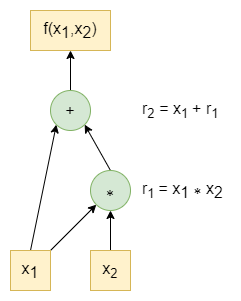
\includegraphics[scale=0.5]{diagrams/forward_example.png}
        \caption{Computational graph of $f(x_1,x_2)\coloneqq x_1+(x_1\times x_2)$}
        \label{fig:forward_graph}
    \end{figure}
    For instance, look at the computational graph in Figure \ref{fig:forward_graph} for $f(x_1,x_2)\coloneqq x_1+(x_1\times x_2)$.
    Now, let us say $x_1=5$, and $x_2=3$, and trace it using the method from Section \ref{sec:tracing}.
    This gives us the trace as \texttt{trace\_result} in Listing \ref{lst:forward_trace}.
    This trace is very straightforward: $x_1$ and $x_2$ are assigned their values, and the multiplication is used in the addition, so it shows up first.
    \begin{haskell}[caption=DSL definition of $f$ and its trace, label=lst:forward_trace, gobble=8]
        f :: Value -> Value -> Expression
        f x1 x2 = ELet "x1" (ELift x1) (
            ELet "x2" (ELift x2) (
                EOp2 Add (ERef "x1") (
                    EOp2 Mul (ERef "x1") (ERef "x2")
                )
            ))

        trace_result :: (TValue, Trace)
        trace_result = (TReal "r2" 20.0, [
            ("x1", TLift (TReal "x1" 5.0)),
            ("x2", TLift (TReal "x2" 3.0)),
            ("r1", TOp2 Mul "x1" "x2"),
            ("r2", TOp2 Add "x1" "r1")
        ])
    \end{haskell}
    Now, let us look at the partial derivatives of $f$ in Equation \ref{eq:reverse_ex}, as we would calculate them using chain rule.
    In Equation \ref{eq:reverse_ex2} we see which calculations we need to perform, we define the partial derivatives or ``adjoints'' of a variable $r_i$ as $\bar{r}_i$.
    We also assume here that the ``seed'' value (the value of $\bar{f}$) is one.
    \begin{equation} \label{eq:reverse_ex}
        \begin{aligned}
            \frac{df}{d\vec{x}}=\nabla f&=\begin{bmatrix}
                \frac{\partial r_2(x_1,r_1)}{\partial x_1}\\
                \frac{\partial r_2(x_1,r_1)}{\partial x_2}
            \end{bmatrix}\tran\\
            &=\begin{bmatrix}
                \frac{\partial x_1}{\partial x_1}+\frac{\partial r_2(x_1,r_1)}{\partial r_1}\cdot\frac{\partial r_1(x_1,x_2)}{\partial x_1}\\
                \frac{\partial x_1}{\partial x_2}+\frac{\partial r_2(x_1,r_1)}{\partial r_1}\cdot\frac{\partial r_1(x_1,x_2)}{\partial x_2}
            \end{bmatrix}\tran\\
            &=\begin{bmatrix}
                1+\frac{\partial r_2(x_1,r_1)}{\partial r_1}\cdot\frac{\partial r_1(x_1,x_2)}{\partial x_1}\\
                0+\frac{\partial r_2(x_1,r_1)}{\partial r_1}\cdot\frac{\partial r_1(x_1,x_2)}{\partial x_2}
            \end{bmatrix}\tran\\
            &=\begin{bmatrix}
                1+1\cdot\frac{\partial r_1(x_1,x_2)}{\partial x_1}\\
                0+1\cdot\frac{\partial r_1(x_1,x_2)}{\partial x_2}
            \end{bmatrix}\tran\\
            &=\begin{bmatrix}
                1+x_2\\
                x_1
            \end{bmatrix}\tran
        \end{aligned}
    \end{equation}
    \begin{equation} \label{eq:reverse_ex2}
        \begin{aligned}
            \bar{f}=\bar{r}_2&=1\\
            \bar{r}_1&=\bar{r}_2\times1\\
            \bar{x}_2&=\bar{r}_1\times x_1\\
            \bar{x}_1&=\bar{r}_2\times1\\
            &+\bar{r}_1\times x_2
        \end{aligned}
    \end{equation}
    With our trace and derivative operations defined, we can now look at how we would get from one to the other.
    It is important to start at the output of the program, and since the trace function we defined in Section \ref{sec:tracing} provides us with the named output, we know where to start on our reverse pass.
    In this case, that would be $r_2$.
    As the final value in the primal calculation is the output of the program, its adjoint will be equal to the adjoint of the program or the seed value.
    This is why Equation \ref{eq:reverse_ex2} posits $\bar{f}=\bar{r}_2$.

    Since we are currently working in reverse execution order, we can just use $\bar{r}_2$ to calculate $\bar{x}_1$ and $\bar{r}_1$ directly.
    It should be reiterated that the trace does not encode any explicit information on the order of operations taken while tracing.
    It is of course a list that was built up one operation at the time, but relying on this forces us to do our reverse pass linearly through the trace, which would prevent some task parallelism opportunities.
    Furthermore, while we can also deduce some order from the naming of the intermediate steps (e.g. $r_1$ was done before $r_2$), we should not do this programmatically, because we wish to reserve parallelism opportunities, but also because some intermediate steps might be hidden in the sub-trace of a map.
    Luckily, we can also discover the ``ancestors'' of any step in the trace by looking at the traced operation.
    For $r_2$ the traced operation was \texttt{TOp2 Add "x1" "r1"}, so we know that for our reverse pass, we next want to look at $x_1$ and $r_1$, as their adjoints (or part of them) rely on the value of $\bar{r}_2$ (which we can also see in Equation \ref{eq:reverse_ex2}).
    For now we will gloss over how we decide which ancestor adjoint to compute first, and just look at the adjoint of $r_1$.
    
    We know that $\bar{r}_1$ is dependent on $\bar{r}_2$, but how exactly is defined by the operation that produced $r_2$, which in this case is addition.
    Now, addition is really simple, as the derivative of addition of two values is the addition of the derivatives of those values.
    See Equation \ref{eq:reverse_add}, where we calculate the adjoint $\bar{r}_1$ and see how this addition just resolves to $1$.
    \begin{equation} \label{eq:reverse_add}
        \begin{aligned}
            \bar{r}_1&=\bar{r}_2\cdot\frac{\partial r_2(x_1, r_1)}{\partial r_1}\\
            &=\bar{r}_2\cdot\frac{\partial(x_1+r_1)}{\partial r_1}\\
            &=\bar{r}_2\cdot\left(\frac{\partial x_1}{\partial r_1}+\frac{\partial r_1(x_1,x_2)}{\partial r_1}\right)\\
            &=\bar{r}_2\cdot(0+1)\\
            &=\bar{r}_2
        \end{aligned}
    \end{equation}

    We can again find the ancestors of $r_1$ by looking at the trace, where we find $x_1$ and $x_2$.
    Let us look at $x_2$ first.
    $\bar{x}_2$ is dependent on $\bar{r}_1$, which we just calculated, but rather than an addition (like $r_2$), $r_1$ is a multiplication.
    We mentioned in Section \ref{sec:bg_ad}, in Equation \ref{eq:dualnumbers}, how the derivative of a multiplication uses both the primal part and the derivative part of a number.
    To get $\bar{x}_2$ we realize (as is visible in Equation \ref{eq:reverse_ex2} as well), that we need the primal value of $x_1$.
    We mentioned before we needed the intermediate values, and this is why.
    Multiplication is not the only operation that requires a primal component, but it is a prime example.
    We see in Equation \ref{eq:reverse_mul} how this adjoint resolves to use the primal component $x_1$.
    \begin{equation} \label{eq:reverse_mul}
        \begin{aligned}
            \bar{x}_2&=\bar{r}_1\cdot\frac{\partial r_1(x_1,x_2)}{\partial x_2}\\
            &=\bar{r}_1\cdot\frac{\partial(x_1\cdot x_2)}{\partial x_2}\\
            &=\bar{r}_1\cdot x_1
        \end{aligned}
    \end{equation}

    Now would also be a good time to quickly reflect on the difference between the tangent (from forward-mode AD) and the adjoint.
    In forward-mode AD, the operation taken to produce some variable, would influence the tangent of that variable.
    This is somewhat intuitive, $r_1$ is a multiplication, and its tangent is $\dot{r_1}=\dot{x_1}\times x_2+\dot{x_2}\times x_1$.
    However, this is not the case for reverse-mode AD.
    In reverse-mode, we see that this information gets passed on to the adjoints of the variable used by the operation, rather than the variable it produced.
    It should be clear why: the tangents denote how the variable is influenced by a change in the inputs, while an adjoint denotes how its corresponding variable influences the outputs.
    It is important to closely observe this, mainly for implementation purposes: we want to calculate (part of) the adjoint before we actually arrive at that step in the trace.
    To calculate $\bar{x}_2$ we need to know what variable $x_2$ was multiplied with (namely $x_1$).
    This means that if we do not want to search through our trace looking for references (to $x_2$ for example) every time, it would be better to calculate (the relevant part of) $\bar{x}_2$ while we still see how it is being used.\\
    This then also bring us neatly to our next conundrum: what if a variable is used multiple times.
    In the example, this goes for $x_1$, something that we have ignored until now.
    The mathematical solution is simple: the partial derivative of a variable that is used multiple times, is just a summation of the adjoints arising from those uses.
    We see this in Equation \ref{eq:reverse_ex2}, where $\bar{x}_1$ is calculated by adding the influence from $r_1$ and the influence from $r_2$ together.
    However, implementation-wise this can be a bit of a hurdle.

    As mentioned, the trace is not in any order.
    This is unlike a typical Wengert list or tape.
    While assuring some order beforehand, or doing topological sort on the computational graph described by the trace, will in large part solve this problem, it also enforces linear execution of the reverse pass.
    And while it is not something we will linger on for now, allowing for concurrency or task parallelism while calculating the derivative might be a nice for a performance boost, and complement the inherent data-parallelism opportunities of array operations.
    So, to solve this, we want to include some form of reference counting.
    During the forward pass we could count how many times each variable is used in the trace.
    Since we need to store intermediate values anyway, keeping a counter for each of these variables seems like little extra work.
    Now, on the reverse pass we can check these reference counters and every time we find part of the adjoint for a variable, we decrement its associated counter.
    If a counter has not reached zero after we have decremented it, we know its adjoint is not yet complete, and we can ignore it for now.
    If it has we can add up all the parts of the adjoint and continue from there.
    This is actually very similar to Kahn's algorithm for topological sorting\cite{kahn1962topological}, except that rather than sorting the graph beforehand, we immediately process the nodes as they become available (have all their incoming adjoints).
    This means we actually do execute the reverse pass in topological order, but by discovering this order as we go it allows us to not strictly do the reverse pass sequentially, something of which we will discuss the merits of further on.
    Provided there is only one output to the program, we know that all reference counters will eventually reach zero, and therefore we are assured we will calculate all adjoints.
    However, this provision is not as clear-cut as it seems.
    Currently our DSL does not really have any room for multiple outputs, and as it is functional does not support any side-effects.
    Instead, to provide multiple outputs, currently the only way is to output an array.
    If we keep arrays in the trace, an array as output would still count as a single value.
    There is a slight discrepancy between the trace and the output if we trace away arrays however: the program will still output an array, but only its individual items are able to be found in the trace.
    This is not really a big problem, since the name of these individual outputs are derived from the name of the full array, but also because it would make little sense to trace away arrays from a program that outputs an array.

    So, we find that our trace needs to be extended with two additional things in the forward pass: intermediate values and reference counters.
    We do this in Listing \ref{lst:forward}, in the data type \texttt{Forward}.
    We also introduce a clone of the \texttt{Traced} data type as \texttt{Forwarded}, as we need to reference the new \texttt{Forward} type in the constructors for maps and vectorized maps.
    We also replace the list structure of \texttt{Trace} with a key-value map.
    This is not strictly necessary, but it allows us to more quickly access the values in the map, while also clearly communicating there is no pre-set order to the trace.
    Each value in a \texttt{Forward} map is a 3-tuple consisting of respectively: the intermediate value, the traced operation performed, and the reference counter for this variable.
    Other than the added reference counting, and saving of intermediate values, the tracing process remains the same as it was in Section \ref{sec:tracing}.

    \begin{haskell}[caption=Forward pass data structures, label=lst:forward, gobble=8]
        data Forwarded
            = FLift TValue
            | FOp0  Op0
            | FOp1  Op1       String
            | FOp2  Op2       String String
            | FMap  [Forward] String
            | FMapV Forward   String

        type Forward = Map String (TValue, Forwarded, Int)
    \end{haskell}

    \subsection{The Reverse Pass}
        As discussed, to facilitate our reverse pass we need both the reference counting and intermediate values.
        Now let us define a function \texttt{reverse} that does the reverse pass.
        This reverse pass should find all the adjoints in the program.
        So, it should take in an object of the \texttt{Forward} type and output a map containing the adjoints.
        In Listing \ref{lst:reverse_def} we define three constructors for adjoints: one for arrays, one for sparse arrays (represented by a single index and the associated value), and one for real values.
        We also define the \texttt{Reverse} type, which will contain these adjoints, and which is returned at the end of the reverse pass.
        The \texttt{Reverse} type maps the names of each part of the calculation to a 2-tuple containing a list of contributions of other adjoints, and its own final adjoint which uses maybe to indicate whether or not it has been calculated yet.

        \begin{haskell}[caption=Definition of the \texttt{Reverse} type, label=lst:reverse_def, gobble=12]
            data Adjoint
                = AArray  [Float]
                | ANull
                | AReal   Float
                | ASparse Int Float

            type Reverse = Map String ([Adjoint], Maybe Adjoint)
        \end{haskell}

        Now before going into precise implementation details we should look at the general picture once more.
        The forward pass provides us with three important components: the final output value of the forward evaluation, the trace on which to do our reverse pass, and the intermediate values we will need to actually calculate everything in the reverse pass.
        First off, the final output value is not actually important for the trace, were it not that it also stores its name in the constructor (for \texttt{TValue}, see Listings \ref{lst:traced} and \ref{lst:language_array}).
        This name points us where to start with the reverse pass, namely the step that produced this output value.

        With our starting point clear, we can now start the reverse pass.
        The programmer will provide some sort of adjoint value (either a real number or an array of them, depending on the output of the regular program), which we will immediately assign to our output value in the reverse pass.
        This makes us ready to actually perform the rest of the reverse pass.

        For any point in the reverse pass the process becomes simple.
        Given some ``current'' point in the computational graph, we look up the adjoint (which should have been established by now) and the forward trace item for this point.
        If the operation in the trace for the current point uses no other values (i.e. has no ``ancestors''), we are done here and return the reverse mapping that contains all the adjoints we have found.
        If the operation does have ancestors, we look at the operation itself to determine how to transform the current point's adjoint for its ancestors.
        If this transformation requires any intermediate values, we can look them up in the forward pass.
        Given the transformed adjoints, we assign these to the adjoint accumulation list for each ancestor.
        We also check if this list now has enough adjoints to match the reference counter in the forward pass.
        If it does not, we are done and can return the reverse mapping.
        However if it does, we add up all the partial adjoints in the list together into the final adjoint and place it in the reverse mapping.
        Then finally, we start the same process for each ancestor of the current node that has its complete adjoint ready.

        Now, let us talk implementation.
        We define two reverse pass functions, \texttt{reverse} and \texttt{resolve}, of which the first will only be a wrapper for the final value and its adjoint to be inserted, and the latter will actually perform the reverse pass.
        Both are shown in Listing \ref{lst:reverse_func}.
        Listing \ref{lst:reverse_func} also introduces two helper functions: \texttt{combineAdjoints} for adding partial adjoints together into the final adjoint of a step in the computational graph, and \texttt{assignAdjoints} for transforming and assigning the adjoints to the ancestors of the current node.
        We will safe the intricate details of \texttt{combineAdjoints} and \texttt{assignAdjoints} for later.
        Finally, we use the \texttt{explore} helper function to try and resolve all the ancestors of the current node as well.

        \begin{haskell}[caption=Definition of the reverse pass functions, label=lst:reverse_func, gobble=12]
            reverse :: String -> Adjoint -> Forward -> Reverse
            reverse s a f = resolve s f $\$$ Map.singleton s ([a], Nothing)

            resolve :: String -> Forward -> Reverse -> Reverse
            resolve s f r = case Map.lookup s r of
                -- Lookup the state of the provided name in the reverse mapping
                -- If its present, but its final adjoint not calculated, we need to check
                -- if we can calculate it
                Just (as, Nothing) -> case Map.lookup s f of
                    -- Find the step taken and the reference counter in the forward pass
                    -- If it is present, check whether or not the adjoint array contains
                    -- items equal to the reference counter (so we know it's all there).
                    Just (fd, c, _) -> if   length as >= c
                                       -- If all partials are present, make the complete
                                       -- adjoint and update the reverse map
                                       then let (a,  r1) = combineAdjoints s f r
                                            -- Then transform and assign the adjoints to
                                            -- the ancestors of this current node.
                                                (r2, sa) = assignAdjoints fd s a f r1
                                            -- Then try all the ancestors as well
                                            in  explore sa r2
                                       -- If we're not ready, just return the current
                                       -- reverse map
                                       else r
                    -- If the named variable isn't present in the forward trace, we've
                    -- got a problem, so we throw an error
                    Nothing         -> error "Variable not in forward trace"
                -- If the adjoint is present, and its final adjoint is already calculated
                -- then we must already be done here, so just return the current reverse
                -- mapping
                Just _             -> r
                -- If the adjoint is missing from the reverse mapping entirely, it's because
                -- we haven't run into it at all yet, so we can also return the reverse mapping
                -- as it is.
                Nothing            -> r
                where
                    -- Applies resolve over a list of ancestors
                    explore :: [String] -> Reverse -> Reverse
                    explore []      r' = r'
                    explore (s':ss) r' = explore ss (resolve s' f r')
        \end{haskell}

        We represent this process on the example program from Figure \ref{fig:forward_graph}, in Figure \ref{fig:reverse_graph}.
        In Figure \ref{fig:reverse_graph} we see the computational graph (forward pass) from Figure \ref{fig:forward_graph} first, as (A).

        Then, with $f=r_2$ as our output value from the forward pass, we can call \texttt{reverse} with some adjoint $a$, the name of $r_2$, and the forward pass we just found to get the reverse graph at (B); this assigns a value to $r_2$ in the reverse map, which we call $r'_2$ in Figure \ref{fig:reverse_graph}.

        As part of the reverse map, $r'_2$ contains two items: a list of partial adjoints (currently only containing $a$), and a final adjoint that has not been calculated yet (so is stored as a \texttt{Nothing}).

        Now we can get into the main loop by calling \texttt{resolve} for $r_2$ with the reverse mapping created by \texttt{reverse}.
        As we can see in graph (C), as we find the partial adjoints $r'_2$ and find that the reference counter in the forward pass is $1=|r'_2|$, we can also call \texttt{combineAdjoints}, which transforms the list of partial adjoints in $r'_2$ to the complete adjoint $a$.

        Then we call \texttt{assignAdjoints} to get graph (D).
        \texttt{assignAdjoints} uses the forward pass to find the ancestors of the current node, in this case $x_1$ and $r_1$, and it also adds the final adjoint of the current node ($r'_2$'s final adjoint is $a$) to their lists of partial adjoints.

        Then \texttt{resolve} on $r_2$ calls \texttt{explore} leading to a \texttt{resolve} call to each of $r_2$'s ancestors, with first up $x_1$ in graph (E).
        However, as we can see from the forward graph (A), we still lack the adjoint from $r_1$ to $x_1$ (highlighted with the red arrow in graph (E)), so we can not resolve $x_1$ yet.

        We leave $x_1$ for later, and this leads us to the resolve call on $r_1$ in graph (F).
        Here we find that $r_1$ does have all its partial adjoints, so we call \texttt{combineAdjoints} to find that the completed adjoint for $r_1$ is also $a$.

        Again, with this adjoint found, we can now call \texttt{assignAdjoints} to bring the adjoint of $r_1$ to its ancestors $x_1$ and $x_2$.
        We will go into how later, but \texttt{assignAdjoints} looks in the forward pass to find that $r_1$ is a multiplication and appropriately transforms $r_1$'s adjoint of $a$ into $a\cdot x_2$ for $x'_1$, and $a\cdot x_1$ for $x'_2$.

        Now in our final steps represented in graph (H), we explore the ancestors of $r_1$, starting with $x_1$.
        We find that we now do have the correct number of partial adjoints for $x_1$, so we can add these together with \texttt{combineAdjoints} to get the final adjoint of $x_1$: $a+a\cdot x_2$.
        Now, after \texttt{combineAdjoints} we call \texttt{assignAdjoints} on $x_1$, however we will find that $x_1$ has no ancestors, which means that $x_1$'s adjoint does not need to be assigned to anything and also that there is no further nodes to explore from $x_1$.

        This means we move back to $r_1$'s explore function, which leads us to $x_2$.
        Here we find again that we can use \texttt{combineAdjoints} to get $x_2$'s final adjoint, and with\\\texttt{assignAdjoints} that $x_2$ has no further ancestors.

        This then moves us back to the end of the explore function in $r_1$, which now finished returns the update reverse mapping to the end of the explore function of $r_2$, which also finishes to return the updated reverse mapping to the original \texttt{reverse} function, and return our reverse pass to the programmer.
        
        \begin{figure}[p]
            \begin{adjustbox}{addcode={\begin{minipage}{\width}}{\caption{%
                Diagram representing the reverse pass process on the example from Figure \ref{fig:forward_graph}.
                }\label{fig:reverse_graph}\end{minipage}},rotate=90,center}
                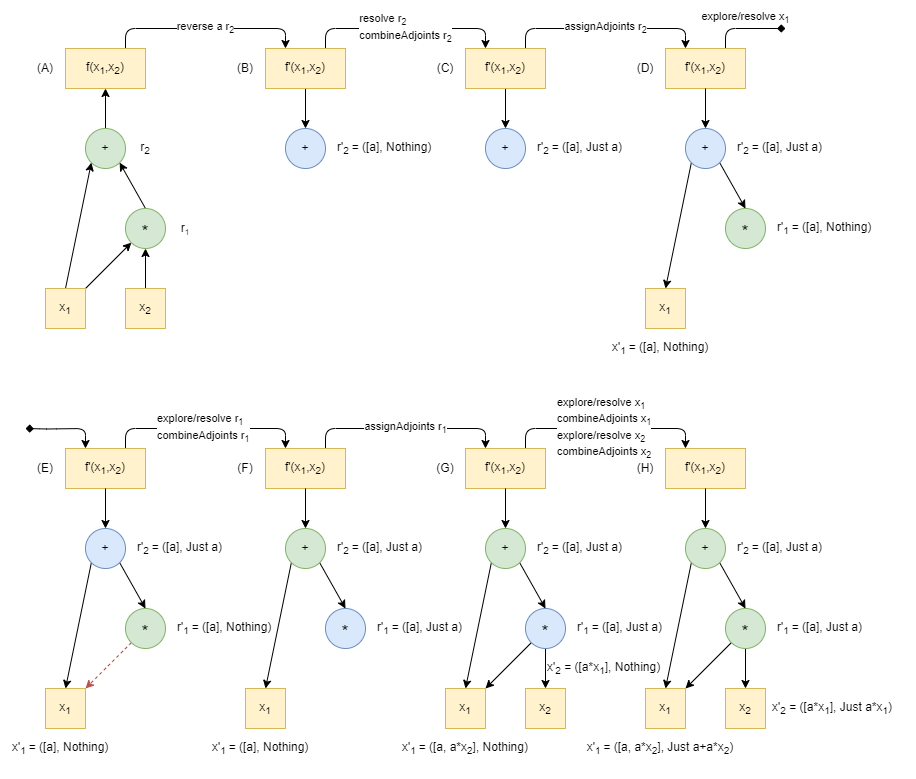
\includegraphics[scale=.6]{diagrams/reverse_example.png}
            \end{adjustbox}
        \end{figure}

        This gives us a global overview of how the reverse pass can be implemented, using the forward pass/trace we have discussed.
        Now there are a couple of questions that remain:
        \begin{itemize}
            \item Can we always add adjoints together?
            \item How do different operations differentiate?
            \item How do we maintain data-parallelism in array operations?
            \item How do we implement task-parallelism on the reverse pass? 
        \end{itemize}
        In the following subsections we will get to all these questions.

    \subsection{Combining Adjoints}
        To go from a list of partial adjoints to a single combined adjoint is not quite as trivial as just adding all together.
        As mentioned before, in Listing \ref{lst:reverse_def}, we defined three types of adjoints, an array, a sparse array, and a real number adjoint.
        The real number adjoint is not complicated, it is the default adjoint and they can be freely added together.
        The difficulty comes in with the array adjoints.
        These adjoints are produced by operations on arrays.
        It will help us to realize now that the adjoint of an array with length $n$, will also have length $n$.
        In reality the adjoint array is no more than an array of adjoints for each item in the original array.

        Knowing this we can start to discover how to add these adjoints together.
        Let us start by discussing adding the sparse and non-sparse array adjoints, as they are almost as simple as adding two real adjoints.
        Since we only add these together as partial adjoint of a single step in the computational graph, we know that the array adjoints whether sparse or not will always have the same length when added together.
        This means we can just add these arrays of adjoints together elementwise, substituting $0$ for all undefined items in the sparse array.

        Only if we add two sparse arrays together, we might need to look up the length of the original array in the forward pass to know the length of these sparse arrays (or we could extend the sparse array constructor to allow for multiple defined items).

        Now the most interesting part comes when we want to add an array adjoint to a real adjoint, or vice versa.
        Namely, there are two ways of doing this, which means that a binary adjoint addition operator is not associative.
        For example, say we find ourselves folding the values in some array $a$ to some real value $b$.
        In the reverse pass, the adjoint of $b$ will be a real adjoint, yet the adjoint of $a$ will have to be an array adjoint.
        Now provided that $a$ has some partial array adjoint (or is represented by an adjoint array filled with zeroes) we must think of a way to add $b$ to the appropriate items.
        Now what these appropriate items in $a$ are, and how $b$'s adjoint needs to be transformed, are of course dependent on the function we fold over array $a$.

        However, we will find that fold takes in an anonymous function, meaning that we need a special case for fold anyways.
        Only for our unary sum operator we perform a fold that is pre-programmed.
        We know that the sum's result is influenced once by each array item, and from the differentiation rules of addition we know that the adjoint of the sum's result is just moved to its ancestors without transformation or touching intermediate values.
        This means that we can just just add the sum's adjoint to each array item.

        The only other way to get from an array to a real value in our language is by using array indexing.
        However this is very simple as well, as indexing does not change anything to the adjoint either.
        Since indexing refers to a specific item in the array, our partial adjoint for the array becomes a sparse array with the incoming adjoint on the indexed position.

        We see the implementation of the helper function \texttt{combineAdjoints} in Figure \ref{lst:combine}, where we also define a binary adjoint addition operator \lstinline{(<+)} to do most of the heavy lifting.
        It should be reiterated that the \lstinline{(<+)} operation adding a real to an array only works because it will only be called by the sum operator.

        \begin{haskell}[caption=Adjoint combination operator and adjoint summation function, label=lst:combine, gobble=12]
            (<+) :: Adjoint -> Adjoint -> Adjoint
            (<+) (AArray as)   (AArray    bs) = AArray (zipWith (+) as bs)
            -- Note: this works because it is only called by sum
            (<+) (AArray as)   (AReal     bs) = AArray (map (+ b) as)
            (<+) (AArray as)   (ASparse i bs) =
                let bs = drop i as
                in  AArray (take i as ++ (b + head bs) : tail bs)
            (<+) (AReal  a)    (AArray    bs) = AReal (a + sum bs)
            (<+) (AReal  a)    (AReal     b)  = AReal (a + b)
            (<+) (AReal  a)    (ASparse _ b)  = AReal (a + b)
            (<+) (ASparse i a) (AArray    bs) = 
                let as = drop i bs
                in  AArray (take i bs ++ (a + head as) : tail as)
            (<+) (ASparse _ _) (AReal     _)  = error "Cannot combine sparse and real
                adjoints, because the length of the sparse adjoint is unknown."
            (<+) (ASparse _ _) (ASparse _ _)  = error "Cannot combine two sparse adjoints,
                because the length of the sparse adjoints are unknown."

            combineAdjoints :: String -> Forward -> Reverse -> (Adjoint, Reverse)
            combineAdjoints s f r =
                -- Get the partial adjoints and combine them together
                let (as, _) = r Map.! s
                    a       = foldr (<+) empty as
                -- And add the completed adjoint to the reverse map
                in  (a, Map.insert s (as, Just a) r)
                where
                    -- Provide an empty identity element
                    empty :: Adjoint
                    empty = case getValue s f of
                        -- Check the intermediate value of s to reveal the right identity element
                        (FArray _ xs) -> AArray (replicate (length xs) 0.0)
                        (FReal  {})   -> AReal  0.0
                        _             -> error "Type mismatch in combineAdjoints/empty"
        \end{haskell}

    \clearpage
    \subsection{Differentiating Operations}
        The actual differentiation rules are applied in the \texttt{assignAdjoints} function, where we take the complete adjoint of a node in the computational graph, transform it according to the operation performed in that node, and then add it as a partial adjoint to its ancestors.
        Its especially the transformation that means we need to write different differentiation rules for almost every operation.

        Let us start with the easy part, the unary and binary mathematical operators.
        In our DSL these are: addition, multiplication, subtraction, and sine.
        Recall that the rules for addition and subtraction are similar, they just transform homomorphically, which means that any adjoint is just ``passed'' to their ancestors without any additional transformation.
        See the examples in Equation \ref{eq:diff_add}.

        \begin{equation} \label{eq:diff_add}
            \begin{aligned}
                \frac{d(x+y)}{dz}&=\frac{dx}{dz}+\frac{dy}{dz}\\
                \frac{d(x-y)}{dz}&=\frac{dx}{dz}-\frac{dy}{dz}
            \end{aligned}
        \end{equation}

        Multiplication and sine are slightly more complicated, both requiring some intermediate value to compute the derivative.
        We have gone over multiplication before, we multiply the incoming adjoint with intermediate value of the other side of the multiplication.
        See the example in Equation \ref{eq:diff_mul}.

        \begin{equation} \label{eq:diff_mul}
            \frac{d(x\cdot y)}{dz}=y\cdot\frac{dx}{dz}+x\cdot\frac{dy}{dz}
        \end{equation}

        The derivative of a sine operation is the cosine on the intermediate value, see Equation \ref{eq:diff_sin}.

        \begin{equation} \label{eq:diff_sin}
            \frac{d(\sin x)}{dy}=\cos x\cdot\frac{dx}{dy}
        \end{equation}

        These are the mathematical operations that we may encounter in the trace.
        Recall that we traced away Booleans, so we do not have to worry about comparison operators.
        With these derivatives cleared up we can now program them into \texttt{assignAdjoints}.
        It is also useful to remember that \texttt{assignAdjoints} should return both the updated reverse mapping, and a list containing the ancestors of the provided node.
        We see the implementation in Listing \ref{lst:assign_simple}.
        This uses another helper function called \texttt{addAdjoint}, which simply just adds the calculated partial adjoint to the list of partial adjoints of the relevant ancestor in the reverse mapping.

        \begin{haskell}[caption={Defining \texttt{assignAdjoints} for sine, addition, subtraction, and multiplication.}, label=lst:assign_simple, gobble=12]
            assignAdjoints :: Forwarded -> String -> Adjoint -> Forward -> Reverse
                -> (Reverse, [String])
            -- Adjoint function for all unary operators (now only showing sine)
            assignAdjoints (FOp1 op s1) _ a f r = case (op, a) of
                (Sin, AReal a') -> case getValue s1 f of
                    -- Take the intermediate value and assign the adjoint to s1, also return
                    -- the list of ancestors: s1
                    (FReal _ x) -> (addAdjoint s1 (AReal $\$$ a' * cos x) r, [s1])
                    _           -> error "Type mismatch in assignAdjoints/FOp1/Sin"
                _               -> error "Type mismatch in assignAdjoints/FOp1"
            
            -- Adjoint function for all binary operators
            assignAdjoints (FOp2 op s1 s2) _ a f r = case (op, a) of
                -- Just add the adjoint to both ancestors
                (Add, _)        -> (addAdjoint s1 a (addAdjoint s2 a r), [s1, s2])
                -- For multiplication, get the intermediate values first
                -- we also deconstruct the adjoint, knowing it is a real number because
                -- (sin x) would return a real number.
                (Mul, AReal a') -> case (getValue s1 f, getValue s2 f) of
                    (FReal _ v1, FReal _ v2) ->
                        (addAdjoint s1 (AReal (a' * v2)) (addAdjoint s2 (AReal a' * v1) r), 
                        [s1, s2])
                    _                        ->
                        error "Type mismatch in assignAdjoints/FOp2/Mul"
                -- Similar to addition, only s2 gets a negative adjoint
                (Sub, AReal a') -> (addAdjoint s1 a (addAdjoint s2 (AReal -a') r), [s1, s2])
                _               -> error "Type mismatch in assignAdjoints/FOp2"
        \end{haskell}

        Another adjoint we should quickly cover is that of array indexing.
        As mentioned before, nothing happens to an intermediate value when it is indexed, so its adjoint will not be transformed either.
        While obvious, the adjoint of the indexed value should only be added to the that specific index in the array's adjoint.
        This is where our sparse adjoint comes in, where we represent a single item in the array without storing anything extra.
        We can see how it is used by \texttt{assignAdjoints} for indexing in Listing \ref{lst:assign_idx}.

        \begin{haskell}[caption={Defining \texttt{assignAdjoints} for the indexing operation}, label=lst:assign_idx, gobble=12]
            assignAdjoints :: Forwarded -> String -> Adjoint -> Forward -> Reverse
                -> (Reverse, [String])
            assignAdjoints (FOp1 op s1) _ a f r = case (op, a) of
                -- Add the sparse array and return the name of the array as ancestor
                (Idx i, AReal a') -> (addAdjoint s1 (ASparse i a') r, [s1])
                $\dots$
            $\dots$
        \end{haskell}

        % NOTE: While an implementation detail, FJoin (also unmentioned in the forward pass) has a simple adjoint too, used by FFold and FFoldV

        \subsubsection{The reverse pass on map operations and function closures}
            Unsurprisingly, the reverse pass is slightly more in-depth on array operations, like map.
            For a regular non-vectorized map, this is still fairly easy to wrap our heads around.
            Especially if we remember that our forward-pass provides us with the following constructor for such maps:
            \lstinline[language=haskell]{FMap [Forward] String}.
            Here we store every application of the mapped function to our array as its own sub-trace.
            Now it becomes easy to realize that the simplest way to reverse-pass over this mapping is just to call the \texttt{reverse} function on each of these forward sub-traces.
            This then provides us immediately with the adjoint of each original array item, which we can combine into an array adjoint for the original array.
            We give this array adjoint as a partial adjoint to the original array (as it is the ancestor of the mapping operation).
            It should be explicitly stated that mapping the \texttt{reverse} function reveals the derivative of a map: another map, but in reverse.

            However, there is a slight obstacle yet to overcome; to do with the mapped function.
            What do we do if the function that is mapped over the array uses variables from anywhere outside the actual array?
            Recall that the functions that are mapped are lambda expressions that have access to any variables in the environment at the function's definition.
            As an example, we can see this expressed in Figure \ref{fig:map_graph}, where some mapped operation on an array $[b]$ uses a variable $a$ to produce the array $[c]$.
            While the partial adjoints for this variable are computed during the reverse pass over every item, they are only stored in the reverse mapping for the particular item.
            And if we extract only the adjoint for the original array item from this reverse mapping, we would throw away these partial adjoints, making it possibly impossible for us to calculate the full reverse-pass of the program, as we will not be able to calculate the adjoint for these outside variables.
            We find that these variables, like $a$ in \ref{fig:map_graph} are ``unofficial ancestors'' of the mapping operation.
            They are used by the mapping operations, but can be a little hard to find, as they are hidden in the sub-traces.

            \begin{figure}[htb]
                \centering
                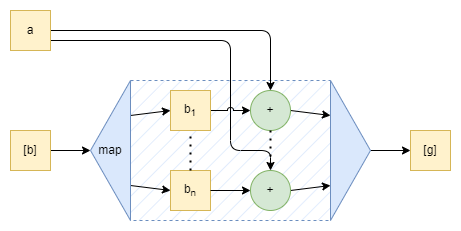
\includegraphics[width=0.6\textwidth]{diagrams/map_example.png}
                \caption{Example of an unofficial ancestor to an array operation}
                \label{fig:map_graph}
            \end{figure}

            Luckily for us the main difficulty with this problem is noticing it.
            Now we know that we have to extract this data into the main reverse pass, we can simply merge the item's reverse pass with the main one.
            We only need to be wary of extracting the partial adjoints for the original map, and combining them together, so we do not overcount the number of partial adjoints against the reference counter of the original array (that in the forward pass only got increased by one for use in the map operation.)
            We see the whole process of finding the adjoint of a map in Listing \ref{lst:assign_map}.

            \begin{haskell}[caption=Implementation of \texttt{assignAdjoints} for the map operation, label=lst:assign_map, gobble=16]
                assignAdjoints :: Forwarded -> String -> Adjoint -> Forward -> Reverse
                -> (Reverse, [String])
                $\dots$
                assignAdjoints (FMap fss s1) s a _ r =
                    let (as, r', ss) = reverseMap fss 0
                        -- Fold sparse adjoints into single array adjoint
                        a' = foldl (<+) (AArray $\$$ replicate (length fss) 0.0) as
                    in  (addAdjoint s1 a' r', Set.toList ss)
                    where
                        reverseMap :: [Forward] -> Int -> ([Adjoint], Reverse, Set String)
                        reverseMap []     _ = ([], r, Set.empty)
                        reverseMap (f:fs) i =
                            let s'  = s ++ '!' : show i
                                rx  = reverse f s' (indexAdjoint i a)
                                -- Extract the array item for 
                                ax  = toSparse i $\$$ fst $\$$ combineAdjoints s' f rx
                                -- Remove items from the original and destination array from this reverse pass
                                -- and add the array items partial adjoint
                                rx' = Map.delete s' (Map.delete (s1 ++ '!' : show i) rx)
                                -- Find the results of the rest of the map
                                (axs, rxs, sxs) = reverseMap fs (i + 1)
                            in  (
                                -- Add this sparse partial to the list
                                ax : axs,
                                -- Add rx' to the main reverse pass
                                Map.unionWith unionReverse rxs rx',
                                -- Add relevant keys to the set of ancestors
                                Set.union sxs $\$$ Map.keysSet rx'
                            )
                        toSparse :: Int -> Adjoint -> Adjoint
                        toSparse i (AReal a') = ASparse i a'
                        toSparse _ _          =
                            error "Type mismatch in assignAdjoints/FMap/toSparse"
            \end{haskell}

            Now with the nonvectorized map taken care of, we can move on to the vectorized map.
            While the idea of finding the adjoint to the map remains the same of course, we now find ourselves with a new problem: a lack of intermediate values.
            Recall that when tracing a vectorized map, we only stored the trace of a single item in the array.
            This was possible because, as we had found the mapped function would not branch, the trace would be the same for each item.
            Now, provided that we did store all intermediate values for this mapping operation, we can perform the same reverse map for the vectorized trace, as with the nonvectorized trace.

            \paragraph*{On Parallelism}
                It should be clear that there is a major inherent parallelism opportunity for each of the mapping operations.
                For the vectorized map this is very clear: data parallelism.
                This is true in evaluation, and is still true in the reverse-pass.
                Namely as the reverse pass is the same for all items, we can use a data parallel mapping function to run the reverse pass in a vectorized manner as well.

                For the nonvectorized map we cannot be sure the operations are the same for each item.
                This means that data parallelism is off the table, however we can still use task parallelism.
                This would not be hard to implement as each item has its own reverse call which can easily be run task parallel.
                Of course, one would need to exercise some caution with the collection of the partial adjoints and reverse maps, but this is not a new problem.
                The combination of the partial adjoints would still need to happen sequentially.

                We will talk more about parallelism when we talk about the reverse map on folds.

        \subsubsection{The reverse pass on fold operations}
            Hello, world!



    \clearpage
    \bibliographystyle{unsrt}
    \bibliography{references}
    \clearpage
    \appendix
    \section{ADT Evaluation} \label{sec:eval}
    In Section \ref{sec:steps}, we introduced an extended lambda calculus.
    In this section we will quickly go over how an evaluator function for this ADT would look like in Haskell.
    We define our evaluator function in Listing \ref{lst:eval}, using the definitions of \texttt{Expression}, \texttt{Value}, and \texttt{Environment} from Listing \ref{lst:language}.

    \begin{haskell}[caption=ADT Evaluator, label=lst:eval, gobble=8]
        eval :: Environment -> Expression -> Value

        eval n (EApply e1 e2) =
                -- Evaluate e1 and e2 first
            let v1 = eval n e1
                v2 = eval n e2
            in  case v1 of              
                    -- Only apply v1 to v2 if v1 is a function as expected
                    VFunc f -> f v2
                    _       -> error "Type mismatch in eval/EApply"

        eval n (EIf e1 e2 e3) =
            -- Evaluate e1 as the condition of the if-then-else statement
            case eval n e1 of
                -- If e1 evaluates to true, evaluate e2
                VBool True  -> eval n e2
                -- Otherwise, evaluate e3
                VBool False -> eval n e3
                _           -> error "Type mismatch in eval/EIf"

        -- For abstractions, we return the function by moving the evaluation into the body.
        -- Where we insert the anonymous value x into the environment as it was when the
        -- function was defined.
        eval n (ELambda s1 e1) = VFunc !*\$ \textbackslash*!x -> eval (insert s1 x n) e1

        eval n (ELift v1) = v1

        eval n (EOp2 op e1 e2) =
                -- Evaluate e1 and e2 first
            let v1 = eval n e1
                v2 = eval n e2
                -- This case syntax allows us to select for the right op with the right
                -- value types at the same time.
            in case (op, v1, v2) of
                (Add, VFloat a, VFloat b) -> VFloat !*\$*! a +  b
                (Equ, VBool  a, VBool  b) -> VBool  !*\$*! a == b
                (Equ, VFloat a, VFloat b) -> VBool  !*\$*! a == b
                (Mul, VFloat a, VFloat b) -> VFloat !*\$*! a *  b
                (Neq, VBool  a, VBool  b) -> VBool  !*\$*! a /= b
                (Neq, VFloat a, VFloat b) -> VBool  !*\$*! a /= b
                _                         -> error "Type mismatch in eval/EOp2"

        -- Resolving references means getting the value from the environment by name.
        eval n (ERef s1) = n ! s1
    \end{haskell}
    \clearpage
    \section{Utility Functions for the Reverse Pass} \label{app:utility}
    The first utility function used in Section \ref{sec:ad}, is \texttt{seedAncestors}.
    It calculates the provides the ancestors of a node in the computational graph with the adjoint of said node.
    The function is given in Listing \ref{lst:seedanc}.
    It uses the function \texttt{getAncestors}, given in Listing \ref{lst:getanc}, which simply gets the ancestors of a specific statement in the trace.
    It also uses two additional functions to combine adjoints, given in Listing \ref{lst:combine}.

    \begin{haskell}[caption=Function for seeding ancestors of a node, label=lst:seedanc, gobble=8]
        seedAncestors :: Forward -> Reverse -> String -> Adjoint -> Reverse
        seedAncestors t r s a = setSeed (getAncestors s) r
            where
                traced :: Forwarded
                (_, traced, _) = t Map.! s

                references :: String -> Int
                references s = v
                    where (_, _, v) = t Map.! s

                setSeed :: [String] -> Reverse -> Reverse
                setSeed []     z = z
                setSeed (s:ss) z = setSeed ss z'
                    where z' = case traced of
                        FOp1 op _ -> case op of
                            Idx i -> case r Map.lookup s of
                                Just (as, _) ->
                                    let as' = ASparse i (toSingle a) : as
                                    in  if   length as' == references s
                                        then Map.insert s (as', combineAdjoints as')
    \end{haskell}

    \begin{haskell}[caption=Function to get ancestors from a node in the trace, label=lst:getanc, gobble=8]
        getAncestors :: Forward -> String -> [String]
        getAncestors f s = case Map.lookup f s of
            Just (_, t, _) -> case t of
                FLift _     -> []
                FOp0  _     -> []
                FOp1  _ a   -> [a]
                FOp2  _ a b -> [a, b]
                FMap  _ a   -> [a]
                FMapV _ a   -> [a]
            Nothing        -> []
    \end{haskell}

    \begin{haskell}[caption=Functions to transform and combine adjoints, label=lst:combine, gobble=8]
        combineAdjoints :: [Adjoint] -> Adjoint
        combineAdjoints [x]     = x
        combineAdjoints (x:y:z) = combineAdjoints (ca x y : z)
            where
                ca :: Adjoint -> Adjoint
                ca (AArray as) (AArray bs)   = AArray (zipWith (+) as bs)
                ca (AArray as) (ASparse i b) = AArray
                    (take index as ++ [as !! index + b] ++ drop (index + 1) as)
                ca (ASparse i b) (AArray as) = AArray
                    (take index as ++ [as !! index + b] ++ drop (index + 1) as)
                ca _           _             = error "Can only sum arrays"
        
        sumAdjoints :: [Adjoint] -> Adjoint
        sumAdjoints [x]     = x
        sumAdjoints (x:y:z) = sumAdjoints (sa x y : z)
            where
                sa :: Adjoint -> Adjoint -> Adjoint
                sa (AReal rx) (AReal ry) = AReal (rx + ry)
                sa _          _          = error "Can only sum singles"

        toSingle :: Adjoint -> Float
        toSingle (AArray vs)   = sum vs
        toSingle ANull         = error "Tried to simplify null adjoint"
        toSingle (AReal v)     = v
        toSingle (ASparse _ v) = v

        toArray :: Adjoint -> Int -> Float
        toArray a@(AArray v) l =
            if   length v == l
            then a
            else error "Array of wrong length"
        toArray ANull        l = error "Tried to make array from null adjoint"
        toArray (AReal v)    l = repeat l v
            where
                repeat :: Int -> Float -> [Float]
                repeat 0 _ = []
                repeat i v = v : repeat (i - 1) v
        toArray (ASparse i v) l = take i zeroes ++ [v] ++ take (l - i - 1) zeroes
            where
                zeroes :: [Float]
                zeroes = 0.0 : zeroes
    \end{haskell}
\end{document}